
% extarticle -> kleiner Schriftgrösse
\documentclass[a4paper, 8pt]{extarticle}
%\usepackage[ansinew]{inputenc} würde umlaute ermöglichen, clashed aber mit babel package :()
%Packages sind in separaten .sty Dateine abgespeichert
\usepackage{include/Vorlage_Cheatsheet}
\usepackage{include/report}
%\usepackage[margin=0.5cm]{geometry}

%\setlist{leftmargin=3mm, nosep}

\title{ZF AEMBS}
\author{Riccardo Degiacomi}
%hello world this is a test for github
%just another test
\begin{document}
% ...stuff goes here....
% 3-column layout
\begin{multicols*}{3}
	\section{SW1 Software und tools}
		\subsection{Design und Architektur}
			\begin{description}
				
				\item[$\bullet$ Mikrocontroller:] Verwendung bei geringem Kosten und Stromverbrauch. Eignet sich für integrierung auf PCB
				\item[$\bullet$ FPGA:] Verwendung wenn mehr Leistung gewünscht als bei $\mu C$ und man Funktionen direkt in HW implementieren möchte (vgl. hoher Stromverbrauch)
				\item[$\bullet$ Embedded Linux:] Verwendung wenn man Netzwerkstacks und Internet nutzen möchte. Bietet grosse Funktionalität. Nachteil; nicht gut für "harte" Echtzeit Anwendungen (langer bootvorgang).
				\item[$\bullet$ Host:] Verwendung bei grossen Systemen. Host ist ähnlich wie PC. Wird oft für GUI und SCADA (Control And Data Acquisition) verwendet.
				
			\end{description}
	Oft werden Systeme als Kombination verschiedener Blöcke Realisiert.\\
	\\
	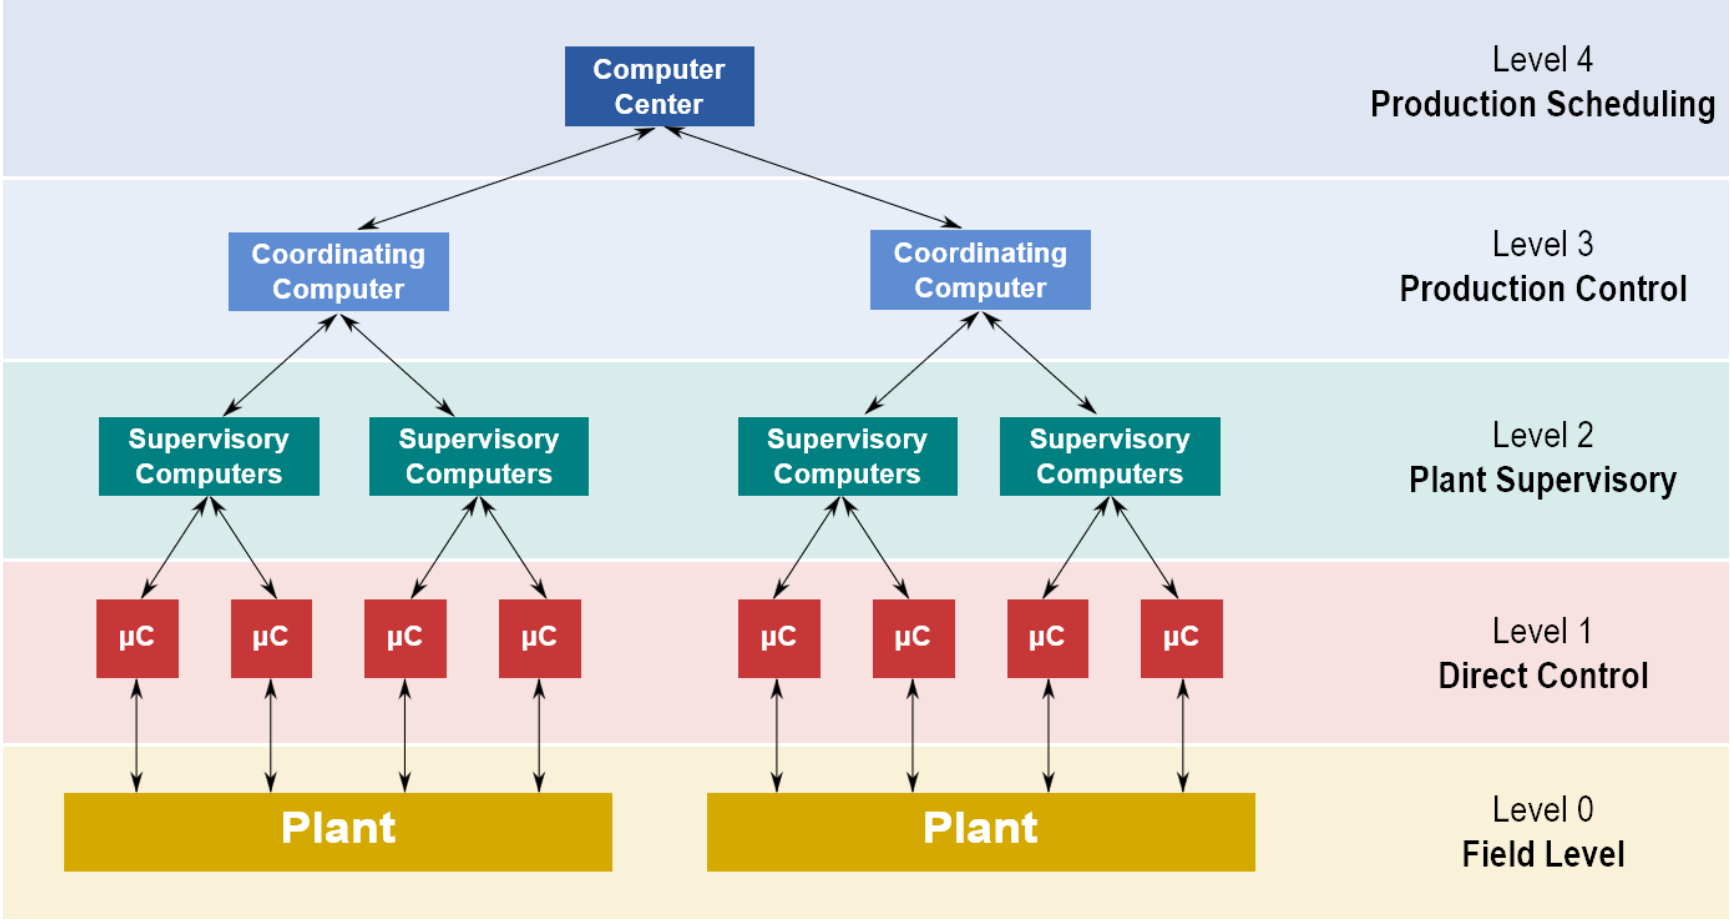
\includegraphics[width=1\linewidth, left]{img/Hardware_Hierarchie}
		\subsection{Crossdevelopment}
		Wenn man nicht auf der selben Entität entwickeln kann spricht man von Host und Target. Auf dem host wird entwickelt, auf dem target ausgeführt. Auf dem Host wird für das Target entwickelt. Dazu nutzt man eine Toolchain.
			\begin{description}
			\item[$\bullet$ Target:] Ist Zielsystem für das entwickelt wird (wofür)
			\item[$\bullet$ Host:] Umgebung auf der entwickelt wird (womit)
			\item[$\bullet$ Toolchain:] Besteht aus Compiler, linker, debugger, standard libraries und anderen Tools
			\item[$\bullet$ Buildumgebung:] Steuert Toolchain und Übersetzungsvorgang. Wird oft mit makefiles gemacht.
			\item[$\bullet$ IDE:] nicht zwingend notwendig\\
			\end{description}

	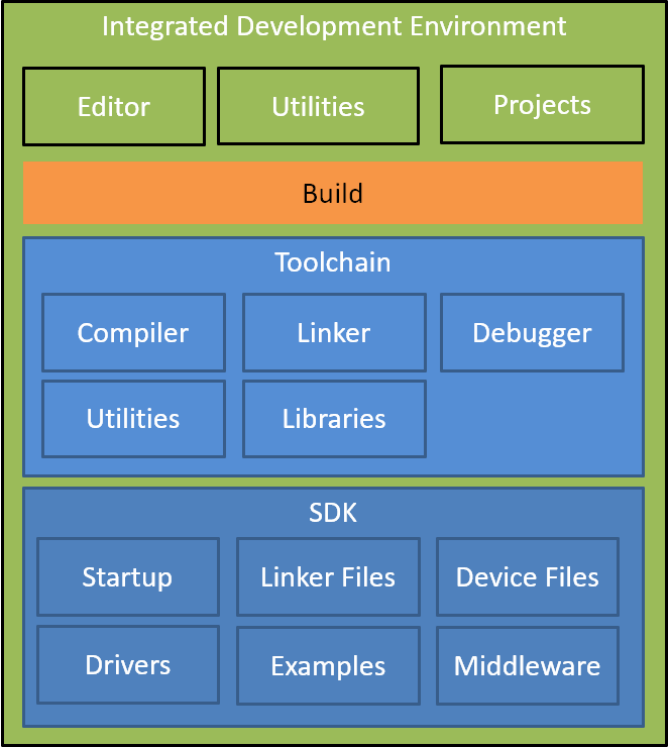
\includegraphics[width=0.9\linewidth,left]{img/Integrated_Development_environement}
	\section{SW2 Software und Device Treiber}
			\subsection{Device Driver}
				\begin{description}
					\item[$\bullet$ Interface:] Abstrahiert von Hardware. Sollte einfach und verständlich sein
					\item[$\bullet$ Synchronisation:] 
					Kann Synchron sein Gadfly, Polling oder asynchron mit Interrupts, Events oder Callbacks (was ist mit snchronisation gemeint dude)
					\item[$\bullet$ Organisation:]
					Einfach: Eine Schnittstellendatei, eine Quelltextdatei (UART,SPI $I^2C$)
					Komplex: Mehrere Dateien mehrere Verzeichnisse  
					\item[$\bullet$ Konfiguration:] Treiber sollte konfigurierbar sein. Gängig ist durch Konfdatei, über Schnittstelle oder mit Makros.
					Siehe:
					https://mcuoneclipse.com/2019/02/23/different-ways-of-software-configuration/
			\end{description}

			\subsection{File Formate}
				\begin{description}
					\item[$\bullet$ ELF/Dwarf:] ist ein Standard Format zur Beschreibung eines ’Executable’
					(Elf) zusammen mit der Debug (Dwarf) Information
					\item[$\bullet$ S19 Motorola S-Record:] Repräsentation der Daten in textueller Form.\\
					Das S19 Format ist ein textuelles und zeilenorientiertes Format, welches
					\colorbox{pink}{’S’ Record ID },\colorbox{yellow}{ Länge },\colorbox{cyan}{ Adresse },\colorbox{green}{ Daten } und eine Checksumme beinhaltet.
					Im Folgenden ein Beispiel:\\
					\colorbox{pink}{S1} \colorbox{yellow}{13} \colorbox{cyan}{7AF0}\\ \colorbox{green}{0A0A0D00000000000000000000000000} 61
					\item[$\bullet$ Intel Hex:]
					Das Intel Hex Format ist auch ein text- und zeilenbasiertes Format, bei
					dem ein Start Code , Länge , Adresse , Typ , Daten und eine Checksumme
					verwendet wird. Nachfolgend auch hier ein Beispiel:\\
					: 10 0100 00 \\214601360121470136007EFE09D21901 40
					\item[$\bullet$ Binary:] Beim Binary Format sind keine zusätzlichen Informationen vorhanden. Bei
					diesem Format sind in der Datei einfach die ’rohen’ Bytes abgespeichert.\newline 
				\end{description}	
	Gemeinsam zu Datei-Formaten von S19, Intel Hex und Binary ist es dass diese
	keine Debug Information enthalten (mussen).\\
	Die benötigen Formate können entweder mit den GNU Werkzeugen direkt
	oder in Eclipse in einem Post-Build Step generiert werden. In der MCUXpresso
	Eclipse IDE können gleich mehrere Formate gleichzeitig in eine Post-Build Step
	erstellt werden
	
	\section{SW3 System}
				\subsection{Systeme}
				%https://www.duden.de/rechtschreibung/integral
				Ein System ist eine Menge von interagierenden oder zusammenhängenden Einheiten, welche ein integrales Ganzes bilden.\\
					\begin{description}
						\item[$\bullet$ Transformierende Systeme:]%beispiel für transformierendes system?							
							Verarbeitet Eingabestrom in Ausgabestrom. Verarbeitet Daten typischer weise kontinuierlich.
							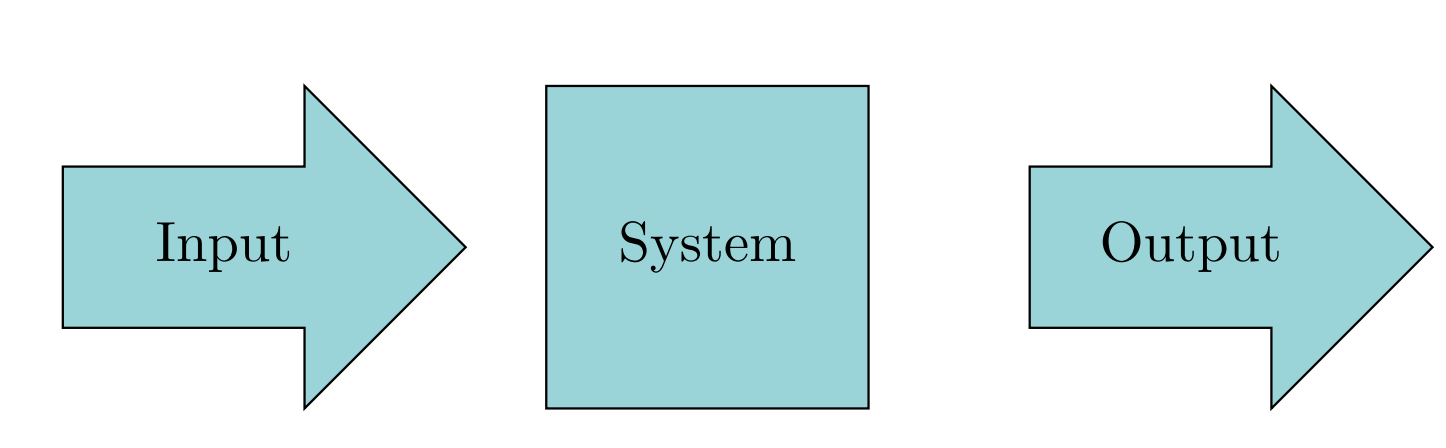
\includegraphics[width=0.8\linewidth,left]{img/Transformierende_Systeme.PNG} 
							\begin{equation}
								O(s)=P(I(s))
							\end{equation}	
							Dabei ist $I()$ eine Eingabe Funktion, $I(s)$ ein Eingabestrom und $P(s)$ die Systemfunktion. Der Eingabestrom
							wird von der Systemfunktion verarbeitet und erzeugt einen Ausgabestrom $O(s)$. Def. \dq Multichannel System\dq: Ein transformierendes System
							mit mehreren Ein- und Ausgabeströmen. 
							\begin{equation}
								O_m(s)=P(I_n(s)) \qquad m,n \in \mathbb{R}
							\end{equation}
							Eigenschaften: Verarbeitungsqualität (gut oder was?), Durchsatz, Systemausnutzung. Benötigen eine gewisse Menge an Speicher. Optimiert auf
							geringen speicherverbrauch. Konflikt mehr speicher schnellere verarbeitungszeit, aber teurer. Sind oft periodische Systeme (Datenlogger, lesen und verarbeiten Daten mit einer gewissen Periode).
						\item[$\bullet$ Reaktive Systeme:]%bsp?								
							Unterscheiden sich zu transformierenden Systemen dadurch, dass Sie auf Ereignisse warten. Sind typischerweise Steuer- und Regelsysteme.
							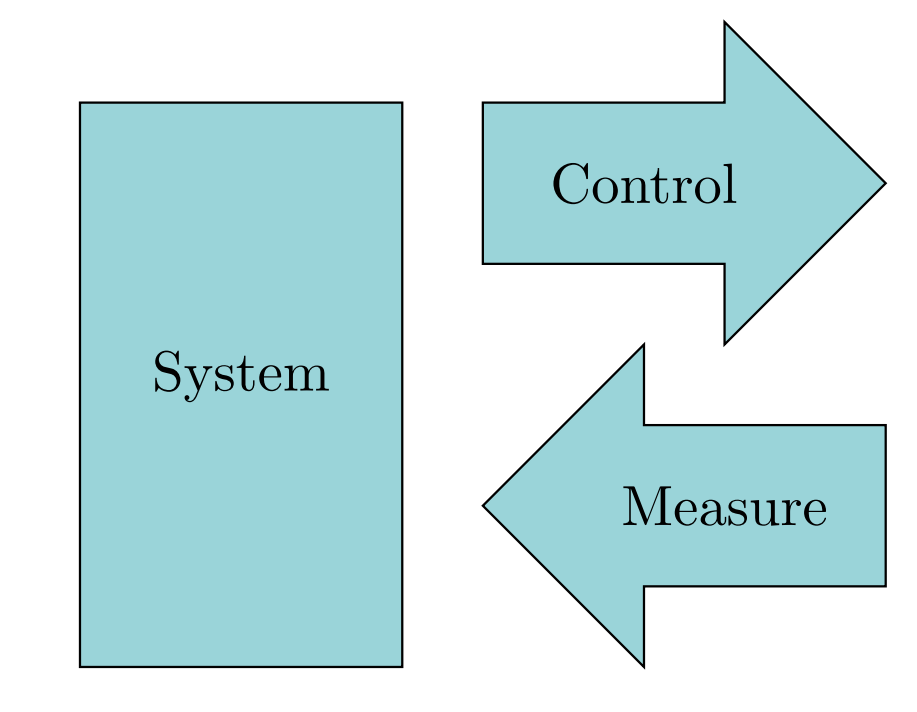
\includegraphics[width=0.6\linewidth,left]{img/Reaktive_Systeme.PNG}
						\item[$\bullet$ Interaktive Systeme:]
							Stellen Schnittstelle zu Benutzer her. Auf kurze Antwortzeit und weil teuer auf hohe auslastung optimiert.
							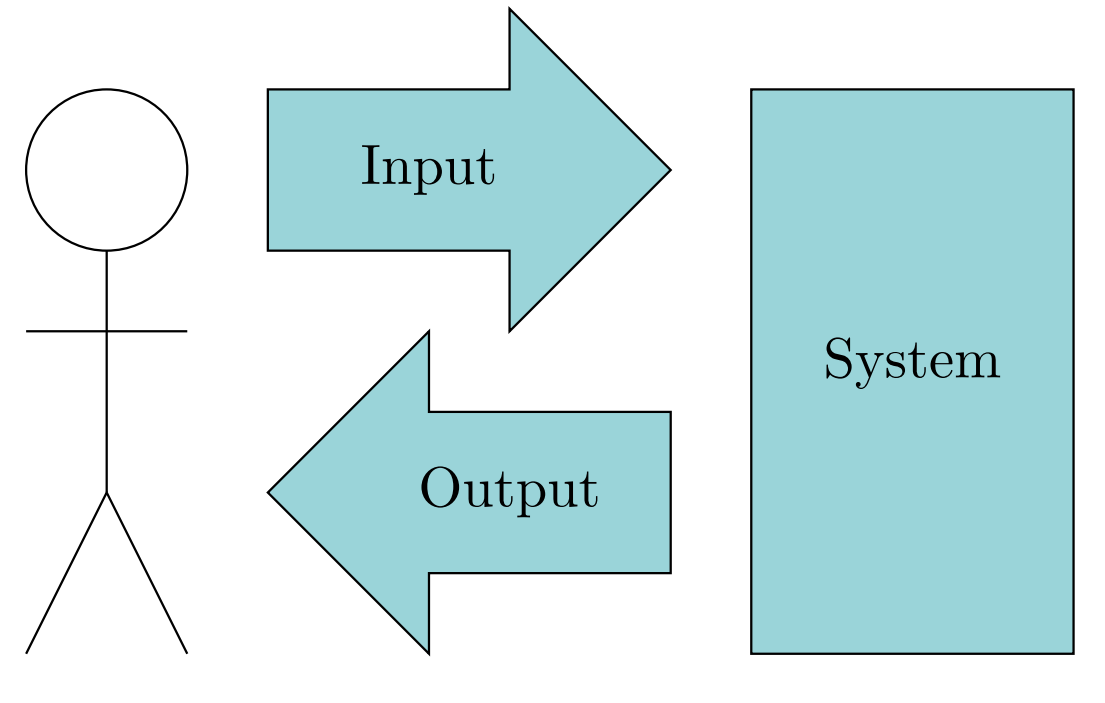
\includegraphics[width=0.6\linewidth,left]{img/Interaktive_Systeme.PNG} 
					\end{description}
		
	\section{SW4 Synchronisation}
					\begin{description}
						\item[$\bullet$ Systeme]
							Computer arbeiten in ihrer eigenen Zeitdomäne. Dies führt zu synchronisationsproblemen mit der Zeitdomäne der echten welt.
							Ein Echtzeitsystem muss die richtige Antwort zur Richtigen Zeit liefern.Timing =  Zeitverhalten, wichtiger Begriff.
							Betrachtet man beispielsweise ein I/O System, stellt man fest, dass dieses nur korrekt funktioniert, wenn Daten zuerst eingelesen und dann gesendet werden.
							Sendet man zu frühm, gehen daten verloren. Um dies zu bewerkstelligen muss man den Ablauf synchronisieren. Es gibt für verschiedene Probleme/Systeme unterschiedliche
							Synchronisationsvarianten.
						\item[$\bullet$ Handshaking]
							Synchronisation für Kommunikation. Ziel ist sicherzustellen, dass eine Meldung empfangen wird. 
							\begin{enumerate}
								\item Empfänger Signalisierten zuerst dass bereit $Rx_RDY$.
								\item Sender legt daten an PORT, Teilt mit dass bereit $DATA_RDY$
								\item Empfänger liest daten, signalisiert dass Daten empfangen $RX_RDY$
								\item Sender bestätigt dies mit $DATA_RDY$ um neuen Zyklus zu beginnen
							\end{enumerate}
							Dieser Prozess wird \dq Handshaking\dq genannt. Wird oft bei Kommunikationsprotokollen verwendet.
							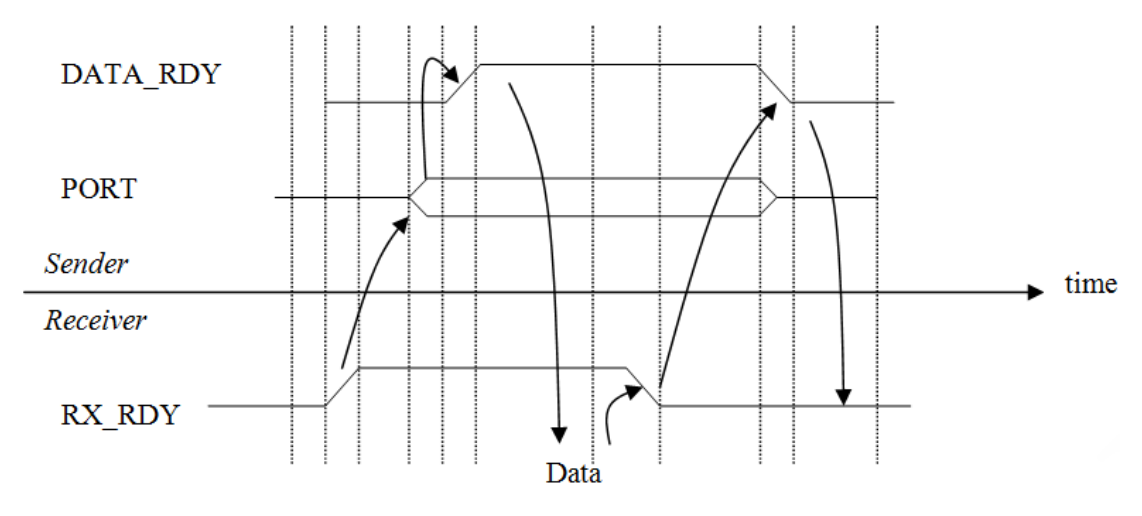
\includegraphics[width=1.1\linewidth,left]{img/Handshaking_Ablauf.PNG}
							\begin{lstlisting}
#define WAIT_TIME 10000
void read(void){
	size_t i;

	PORTB.DDRO = 1; /*pin B0 as output pin*/
	for(i=0; 9<sizeof(buffer); i++) {
		int j;
		PORTB.B0 = 1; PORTB.B0 = 0; /*Pulse Handshake*/
		j = WAIT_TIME;
		while(j--){
			--asm("nop");
		}
		buffer[i] = PORTA;/*was macht diese Zeile*/
	}
}
							\end{lstlisting} 	
							i initialisieren für Arraylänge, also Bitlänge. PortB als Output definieren, Was macht dieses struct? In der For Schlaufe wird B0 kurz auf high und dann auf Low gesetzt.
							Es wird also ein sehr kurzer Puls ausgesendet (woher weiss ich wie lange der Puls andauert?).Danach wird dann jeweils eine kurze Zeit gewatet, Befor dann die Daten des Port A
							eingelesen werden. Welche Rolle hat hier PORTA, ist das die Schnittstelle wo informationen empfangen werden?
							\begin{lstlisting}
void read(void){
	size_t i;

	PORTB.DDR1 = 1;/*pin B1 as output pin*/
	PORTB.B1 = 1;/*B1 initially high*/
	for(i=0; i<sizeof(buffer); i++){
		PORT.B1=0;/*initiate handshaking with setting B1 low*/
		while(!PORT.B0){}
		while(PORT.B0){}/*synchronize*/
		buffer[i]=PORTA;
		PORTB.B1=1;/*end handshake*/
	}
}
							\end{lstlisting}
							Das Programm ist eine Erweiterung des ersten. B1 wird auf 1 gesetzt. Daten sollen nicht gesendet werden. Danach wird B1 auf 0 gesetzt.
							Daten sollen empfangen werden.Solange B0 auf 0 ist soll gewartet werden. Wenn B0 auf 1 geht soll gewaret werden, bis B0 wieder auf 1 ist.
							Es soll also gewartet werden, bis ein Puls von B0 gesendet und empfangen wurde. Danach wird in das Array geschrieben. Aber ich verstehe nicht weshalb B0 nicht 
							nochmals in diesem codebeispiel implementiert wurde. Man müsste schon die beide Beispiele irgendwie vereinen, oder? Und wird jetzt für jedes Zeichen das gesendet
							wird, ein Puls ausgesendet? Wie wird geregelt, dass das richtige bit eingelesen wird beim lochkarten beispiel?Wie könnte die Synchronisation beim lochkarten beispiel
							in pseudocode aussehen?
						\item[$\bullet$ Realtime Synchronisation]
							Ist ein Weg ein Programm zu verzögern. Die Methode heisst Realtime weil sie eine Echte Zeit wartet um zu synchronisieren.
							\begin{lstlisting}
void read(void){
	size_t i;

	for(i=0; i<sizeof(buffer); i++){
		for(int j=0; j<10000; j++){
			/*wait some time*/
		}
		buffer[i]=PORTA;
	}
}								
							\end{lstlisting}
							Bei diesem Programm beispiel wird in der äusseren for-Schleife jeweils in das Array geschrieben. Diese zu durchlaufen benötigt
							Zeit. Diese Zeit ist inhärent. Die innere Schleife dient dazu explizit Zeit zu verbraten, diese Zeit nennt man explizit. Die innere
							Schleife gibt dem PortA etwas mehr Zeit etwas in den Buffer zu schreiben. Ist die Wartezeit an die Geschwindigkeit des Motors angepasst
							so kann man erfolgreich Daten einlesen. Das Beispiel unten wäre eine noch verfeinerte Variante.
							\begin{lstlisting}
void read(void){
	size_t i;

	for(i=0; i<sizeof(buffer); i++){
		for(int j=0; j<10000; j++){
			--asm("nop")
		}
		buffer[i]=PORTA;
		}
}																
							\end{lstlisting}
							Man kann auch einfach eine Wartefunktion mit einem Timer erstellen und diese verwenden.
							\begin{lstlisting}								
void read(void){
	size_t i;

	for(i=0; i<sizeof(buffer); i++){
		WaitMs(500):
		buffer[i]=PORTA;
	}
}
							\end{lstlisting}							
						\item[$\bullet$ Gadfly Synchronisation aka Polling]
							Bei der Realtimesynchronisation wartet man länger als nötig, bei der Gadfly synchronisation wird dies vermieden.
							Man überprüft periodisch einen Zustand und fährt
							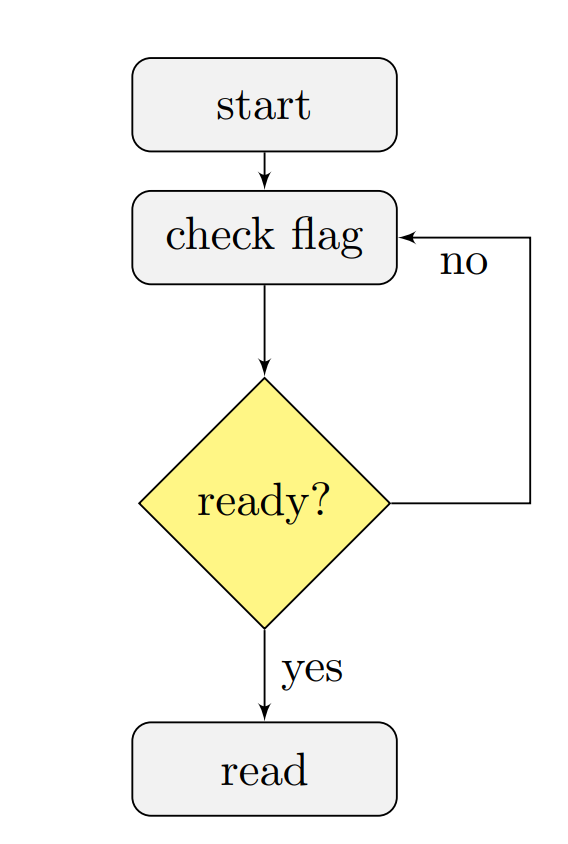
\includegraphics[width=0.6\linewidth,left]{img/gadfly_loop.PNG}
							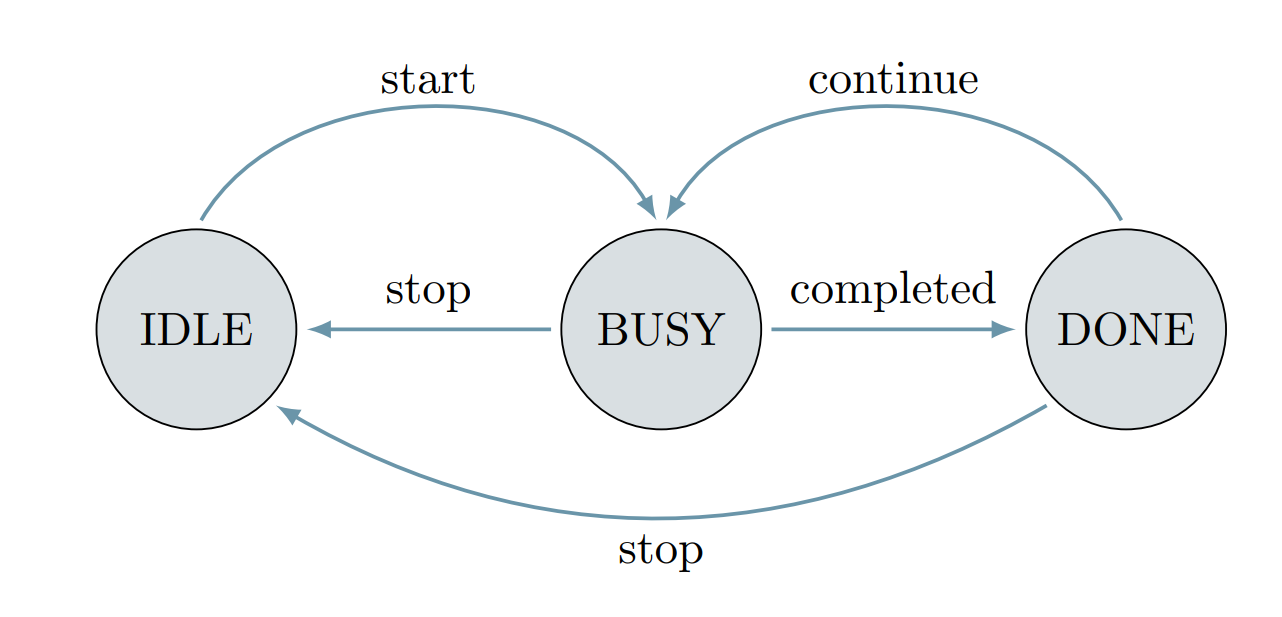
\includegraphics[width=0.6\linewidth,left]{img/gadfly_zustandsdiagramm_device.PNG}
							Codebeispiel Gadfly für Lochkartenleser:
							\begin{lstlisting}
void read(void) {
	size_t i;

	for(i=0; i<sizeof(buffer); i++){
		while(!PORTB.B0){
		/*solange eine Null anliegt wird gewartet
		Null=kein Loch*/						
		}
		buffer[i]=PORTA;
		while(PORTB.B0){
		/* es wird gewartet bis wieder eine Null kommt 
		also bis das Loch den Sensor ueberquert hat */						
		}
	}
							\end{lstlisting}  
							Hier wird gleich zweimal mit Gadfly synchronisiert, oder?
						\item[$\bullet$ Gadfly Synchronisation aka Polling]
							Realtimesync. und Gadflysync. haben den Nachteil, dass diese Rechenzeit auf der CPU oder der MCU verwenden.
							Die Interruptsync. umgeht dieses Problem. Die idee ist, dass man eine Anfrage startet und dann asynchron benachrichtigt 
							wird.
							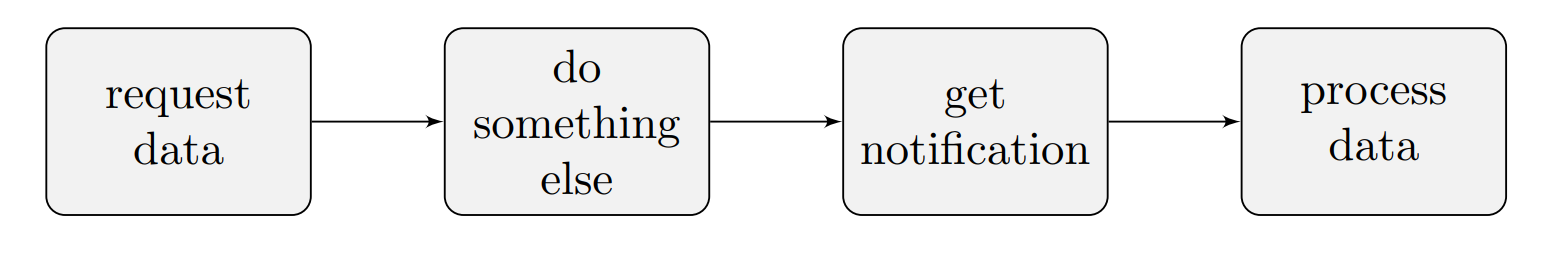
\includegraphics[width=0.6\linewidth,left]{img/interruptsync_1.PNG}
							Interrupts sind in die Logik der Hardware eingebaut. Es ist wichtig dass man sich bewusst ist, dass beim auslösen 
							eines Interrupts etliche operationen automatisiert ablaufen.
							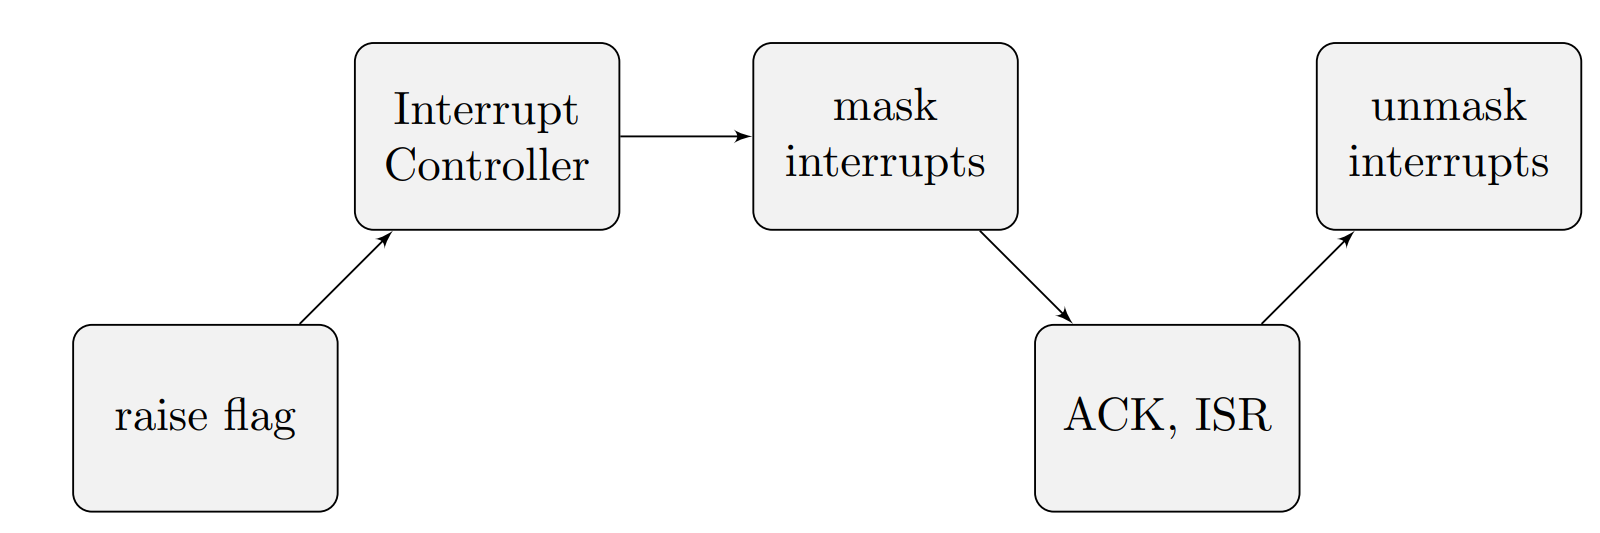
\includegraphics[width=0.6\linewidth,left]{img/interruptsync_2.PNG}
							Zudem ist es wichtig zu wissen, dass nicht alle Coreregister auf dem Stack gespeichert werden können. Dies hat zur Folge dass
							der Programmierer oder der Compiler die Statusrettung der  betroffenen Register ermöglicht wird.  Das eintreten und Verlassen der Interrupts 
							ist atomar, also ohne unterbrechung
							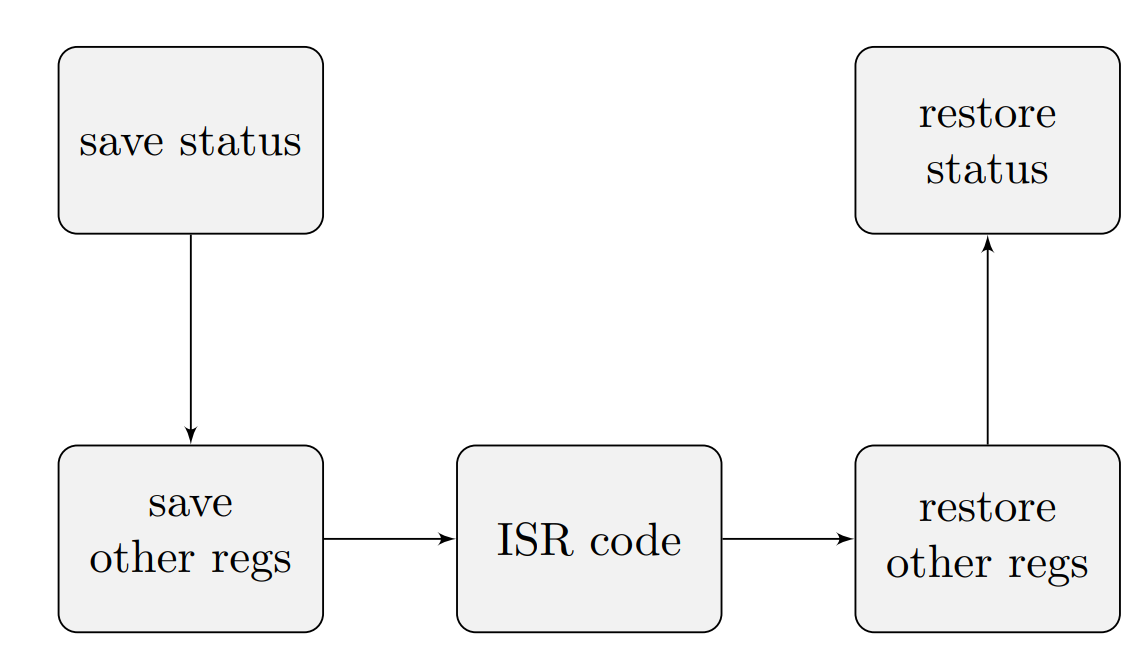
\includegraphics[width=0.6\linewidth,left]{img/interruptsync_3.PNG}
							Beispiel Code für Parkticket leser. 
							\begin{lstlisting}
volatile bool isrFlag=false;
void GPIO_ISR(void){
	AcknowledgeInterrupt
	isrFlag=true;
}

void read(void){
	size_t i;

	isrFlag=false;
	ConfigureGPIO(rising_edge);
	EnableInterrupt(gpio_isr);
	for(i=0; i<sizeof(buffer); i++){
		while(!isrFlag){};
		buffer[i]=PORTA;
		isrFlag=false;
	}
}
							\end{lstlisting} 	
							Es kann nur in den Buffer geschrieben werden sobald ein Interrupt ausgelöst wurde. Die interruptroutine setzt einfach das isrFlag auf true.
							In C und C++ spezifiziert volatile, dass sich der Wert der Variable jederzeit ohne expliziten Zugriff im Quelltext ändern kann.	Zudem verhindert volatile 
							dass die Variable vom Compiler wegoptimiert wird. Das Programm greift somit immer auf den in der Hardware vorhandenen Wert zu. Daher kann diese Variable
							dazu verwendet werdenm, den Prozess zu synchronisieren. Wichtig ist, die ISR sollte allgemein immer sehr schnell abgearbeitet werden, damit diese
							Keine anderen ISR mit tieferer Priorität blockiert.	Wenn ich nicht in der Interrupt Routine etwas mache, sondern nur ein Flag setze, wo 
							ist dann der Unterschied zum Polling?
						\item[$\bullet$ GPIO Interrupts]
							Mit dem Software Development Kint (SDK) kann man Interrupts auch auf den GPIOs verwenden. Man muss dazu den Pin bzw. ein GPIO Port 
							auf Input schalten und die ISR definieren. Der Code Hierfür könnte wie folgt aussehen:
							\begin{lstlisting}
void PORTB_IRQHandler(void){
	GPIO_PortClearInterruptFlags(BOARD_BUTTON_DOWN_GPIO, 1U<<BOARD_BUTTON_DOWN_PIN);
}

void main(void){
	gpio_pin_config_t sw_config = {
		kGPIO_DigitalInput, 0,	
		};
		GPIO_pinInit(BOARD_BUTTON_DOWN_GPIO, BOARD_BUTTON_DOWN_PIN, & sw_config);
		PORT_SetPinInterruptConfig(BOARD_BUTTON_DOWN_PORT, BOARD_BUTTON_DOWN_PIN, kPORT_InterruptFallingEdge);
		EnableIRQ(PORTB_IRQn);
}
							\end{lstlisting} 	
					\end{description}
	\section{SW5 RTOS}
		Um Echtzeitbedingungen einhalten zu können, benötigt man ein RTOS. Weiterhin kann man mit Hilfe eines RTOS das System erweitern ohen die 
		Komnplexität massiv zu erhöhen (Skalierbarkeit).
				\begin{description}
					\item[$\bullet$ Realität]
						Def: Echtzeit-Systeme können für die echte Welt benutzt wreden.
						Echtzeit ist eine Anforderung an ein System. Diese Anforderung kann an alle Systemklassen (transformierend, reaktiv und interaktiv)
						gestellt werden.
					\item[$\bullet$ Rechtzeitigkeit]
						Ein Rechnersystem unterscheidet zu anderen Systemen. Ein Rechner ist getaktet und alles passiert synchron mit dem Clock. 
						Ein Rechnersystem ist über Aktuatoren und Sensoren mit der echten Welt verbunden. 
						Ein Echtzeitsystem muss zur richtigen Zeit agieren können (Richtigzeit wäre besser). Was richtig ist, hängt von der Anwendung ab.
						\begin{itemize}
							\item Absolute Rechtzeitigkeit Einschalten der Bewässerung jeden Tag zur gleichen Zeit 
							\item Nachdem festgestellt wurde, dass der Gartenboden trocken ist, soll in der darauf folgenden Nacht zum Zeitpunkt
							xy die bewässerung für eine gewisse Zeitspanne laufen. 
						\end{itemize}
					\item[$\bullet$ Echtzeit für Rechner]
						Ein echtzeit System muss zur richtigen Zeit das Richtige tun.
					\item[$\bullet$ Echtzeit für Rechner]
						 Ein Echtzeitsystem ist ein System, dessen Richtigkeit der Berechnungen nicht nur von der Logischen korrektheit der Rechnung
						 abhängt, sondern auch vom Zeitpunkt zudem die Rechnung produziert wurde. Wenn die zeitlichen Rahmenbedingungen nicht eingehalten werden
						 können, so spricht man von einem System Fehler. Das bedeutet also, dass man beweisen muss, dass das richtige Resultat zur richtigen Zeit
						 aufgetreten ist. Wichtig, die Geschwindigkeit eines Rechners ist nicht konstant. Ein Computer ist als Echtzeitsystem klassifiziert, wenn er
						 auf externe Ereignisse in der echten Welt reagieren kann: mit dem richtigen
						 Resultat, zur richtigen Zeit, unabh¨angig der Systemlast, auf eine deterministische und vorhersehbare Weise. Dies kann man nur sicherstellen wenn 
						 man zu jedem möglichen Zeitpunkt mit den jeweils gegenwärtigen Informationen des Systemzustandes bestimmen kann, was der nächste Systemzustand sein wird.
						 Problematisch ist dabei, dass wenn ein Prozess die Zeitbedingung nicht einhalten kann, das ganze System diese dann auch nicht einhalten kann.s
					\item[$\bullet$ Harte und weiche Echtzeit]
						Von harter Echtzeit spricht man, wenn durch das Nichteinhalten der Zeitvorgabe das System als nicht Funktionsfähig deklariert wird. Bei weicher 
						Echtzeit führt ein Nichteinhalten der Zeitvorgabe zu einer Degradierung.(Bsp. Video Encoder)
					\item[$\bullet$ Periodische Echtzeit]
						Ist das Verwendete System sehr schnell, so kann man verschiedene Dinge quasi gleichzeitig erledigen.
							\begin{lstlisting}
for (;;) {
	if ( time ==530) { /* start at 05:30 am */
		StartIrrigation () ; /* turn relay on */
	} else if ( time ==535) { /* stop at 05:35 am */
		StopIrrigation () ; /* turn relay off */
}
							\end{lstlisting}
						Da dies einen $\mu C$ kaum auslastet, kann man noch weitere Funktionen einfügen.
							\begin{lstlisting}
for (;;) {
	if ( time ==530) { /* start at 05:30 am */
		StartIrrigation () ; /* turn relay on */
		}
	if ( time >530 && time <535) { /* irrigate from 05:30 am to 05:35 am */
/* control the water pump , needs to be called every 10 ms: */
		ControlIrrigation () ;
		WaitMs (5) ; /* wait 5 ms ( additional 5 ms will be added ) */
	}
	MeasureHumidity () ; /* needs to be called every 5 ms */
	WaitMs (5) ;
	if ( time ==535) { /* stop at 05:35 am */
		StopIrrigation () ; /* turn relay off */
	}
}
							\end{lstlisting} 						
				\end{description}
		\section{SW6 FreeRTOS}
			\subsection{FreeRTOS Lizenz}
				War zu Beginn unter modifizierter GNU GNU Public License erhältlich. Nach Übernahme von Amazon wurde diese aber
				in eine MIT Lizenz umgewandelt.
				\begin{itemize}
					\item Keine Kostenfolge
					\item Keine Einschränkungen
					\item Kann: Kopieren, ändern, einbinden, publizieren, berteilen, sublizenzieren, verkaufen
					\item Copyright und Bedingungen müssen unverändert weitergegeben werden
				\end{itemize}
			\subsection{Distributionen}
			FreeRTOS hat seine offizielle Web Seite auf http://www.freertos.org und kann
			von dort auch heruntergeladen werden. Abbildung 5.6 zeigt die "ubliche Struktur
			der Dateien. FreeRTOS und seine Dateien ist auch auf SourceForge oder seit
			2020 auch auf GitHub verfügbar.
			Von der Hochschule Luzern ist eine Portierung von FreeRTOS im McuOnEclipse SourceForge Projekt verf"ugbar. Dies ist eine Version welche im gleichen 
			Port mehrere Mikrocontroller Architekturen unterstutzt (S08, S12(X), S12X,
			phische Konfiguration mittels Processor Expert (Abbildung 5.8. Diese Version
			verf"ugt "uber eine Shell, Low Power Timer und Tickless Idle Unterst"utzung mit
			zus"atzlichen RTOS Tracing Funktionen wie z.B Percepio Tracealizer und Segger
			SystemViewer. Eine Version ohne Processor Expert ist auf GitHub im McuOnEclipseLibrary Projekt verf"ugbar.
			\subsection{Architektur}
				\begin{description}
					\item[$\bullet$ Philosophie]
						Der Kernel ist sehr klein und benötigt nur wenige Dateien.Ist überwiegend in C formuliert, teile des Interrupthandlings
						sind in Assembler.Kann auch mit einer Anwendung in C++ benutzt werden(was heisst das?).Der Kernel ist statisch konfiguriert.
						Dies bedeutet, dass sich die meisten Einstellungen in einer HeaderDatei (FreeRTOSConfig.h) modifizieren lassen.	Dies bedeutet, dass der 
						Kernel statisch auf die Anwendung abgestimmt ist(Wicht wie beispielsweise eine Library).
						\begin{itemize}
							\item Preemtive Scheduling 
								Es Läuft immmer der Task mit der höchsten Priorität. Tasks mit gleicher Priorität teilen sich die Rechenzeit
								(fully preemptive with round robin time slicing-> alte was?) 
							\item Cooperative Scheduling 
								Ein Kontext Switch (Was isch en kontegschd switsch?) findet nur statt wenn ein Task blockiert oder explizit ein ’Yield’ aufruft. Ein ’Yield’ ist die Auforderung an
								den Kernel, einen Kontext Switch vorzunehmen.\\
						\end{itemize}
						Der Kernel benötigt im Prinzip nur zwei Interrupt arten:\\
						\begin{itemize}
							\item Tick Interrupt
								einen periodischen Interrupt welcher einen Kontext
								Switch (Preemption) ausl"osen kann und welcher dazu dient, einen Z"ahler
								(Tick Counter) fur die Zeitbasis nachzuf"uhren. Für Cortex-M ist dies meis der SysTick.
							\item Software Interrupt 
								ein interrupt welcher vom Kernel ausgel¨ost werden
								kann um einen Kontext Switch zu veranlassen.	 
						\end{itemize}
						Der Tick Interrupt wird als timing base genutzt. Der Kernel zählt nicht in Sekunden, sondern in Ticks. Mit dem TickInterrupt kann man eine
						beliebeige Zeitverzögerung generieren. Wenn Beispielsweise ein Tickinterrupt 10 millisekunden benötigt und man möchte einen Task um 500 Millisekunden 
						verzögern, dann benötigt der Kernel 50 Ticks. Das Tickinterrupt beeinflusstdas timing des ganzen kernels. Typische tickinterrupt perioden sind 10ms oder 1ms 
						.Eine  schnellere tickinterrupt periode erhöht die Interruptload auf ein System, dies ist zu berücksichtigen. FreeRTOS unterstützt eine Tickinterrupt Periode
						von bis zu 1kHz. FreeRTOS hat immer einen Laufenden Task, den IDLE Task.RTOS verwendet normale globale variablen für den eigenenen 
						state und den kernel. Für die Liste der verfügbaren task descriptors werden globale pointer genutzt. Alle anderen dynamischen Daten die zur Laufzeit erzeugt 
						werden, sind im Heap. Der heap ist ein memorypool um speicher zur laufzeit dynamisch zu allozieren. Die Taskpriorität nimmt nimmt mit zunehmenden Zahlen zu. Der IDLE
						TASK wäre dementsprechend 0. Es ist Möglich Tasks zur Laufzeit zu erstellend und löschen. Jeder Task hat seinen eigenen context, stack und stack variablen.
						Auf den Cortex-M modellen wird der Main Stack Pointer für die interrupts verwendet, und der Process Stack Pointer für die Tasks verwendet. Das Betriebssystem
						verwendet softwareinterrupts um zwischen tasks zu wechseln. Task stacks sind designed wie interrupt stacks. Wird also ein neuer Task gestartet, geschieht dies gleich
						wie beim Rückkehren eines Interrupts (was auch immer das heissen soll). Tasks laufen typischer weise in einer endlos for-Schleife.
							\begin{lstlisting}
static void MyTask ( void * params ) {
	( void ) params ; /* not used */
	for (;;) {
		/* do the work here ... */
	} /* for */
	/* never return */
}
							\end{lstlisting} 
						Tasks laufen bis sie von einem anderen Task beendet werden. Die einzige ausnahme ist wenn sich ein Task selbst beendet.
							\begin{lstlisting}
static void SuicideTask ( void *params ) {
	( void ) params ; /* not used */
	/* do the work here */
	vTaskDelete ( NULL ); /*killing myself*/
	/*won't get here since i am dead :D*/
}
							\end{lstlisting} 
						RTOS wird mit $vTaskStartScheduler()$ gestartet. Diese Funktion kreiert dann auch gleich den IDLE task. Der IDLE task hat die Priorität $tskIDLE_PRIORITY$,
						also null und führt unterhaltungs und instandhaltungs aufgaben aus für den Kernel.
					\item[$\bullet$ Block Diagramm]
						Das Betriebssystem benötigt lediglich 10 source files und die entsprechenden Headerfiles.
						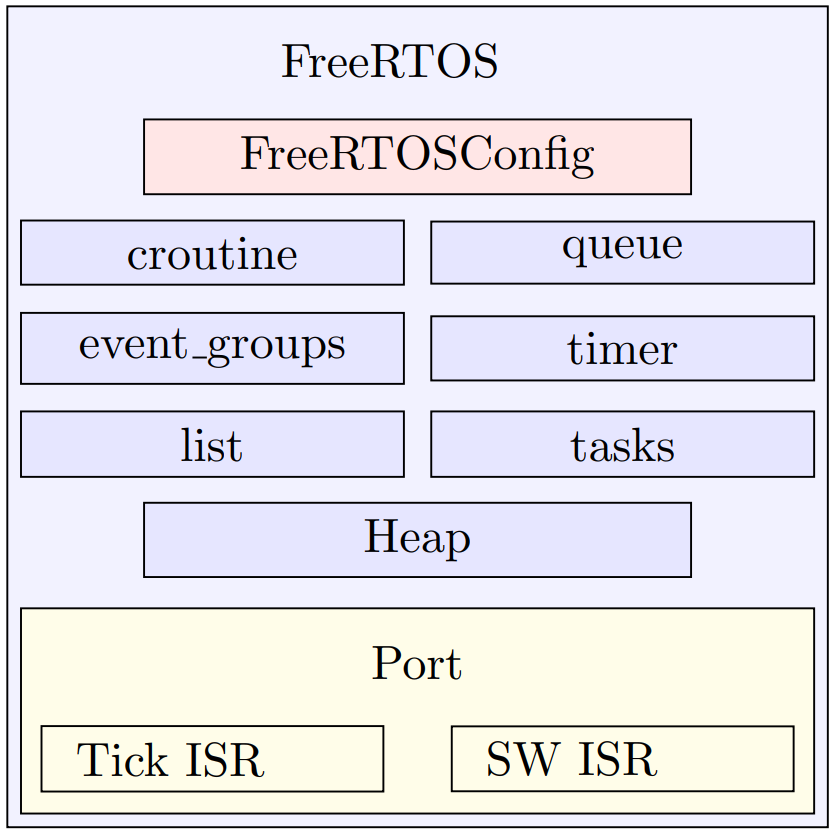
\includegraphics[width=0.6\linewidth,left]{img/FreeRTOS_Achitecture.PNG}			
						\begin{itemize}
							\item FreeRTOSconfig ist ein header file mit makros zur Konfiguration der Einstellungen des Betriebssystems.
							\item croutine implementiert Co-Routinen support in croutine.c. Co-routinen sind mini-threads welche denselben Task teilen.
							\item  event\_groups impementieren support für event flags in event\_group.c 
							\item list in list.c implementiert ein list handling welches intern von RTOS genutzt wird (BSP. für eine liste wartender objekte)
							\item queue ist ein modul welches die queue, semaphore und mutex unterstützung(WTF?) implementiert
							\item timer wwird genutzt um die timer zu implementieren (timer.c).
							\item task implementiert den scheduler in task.c
							\item heap ist ein heap manager und heap speicher. Es werden verschiedene implementationsvarianten angeboten (heap\_1.c, heap\_2.c ...)
							\item Port implementiert RTOS für eine bestimmte architektur, Mikrocontroller und toolchain. Port ermöglicht RTOS den zugang zu Hardware
								  Funktionalitäten. Enthält implemenation Tickinterrupt und SoftwareInterrupt.
							\item Zusätzlich gibt es noch middleware für FreeRTOS (unter einer anderen Lizenz). Beispielsweise Trace,file systems, oder commmand line interface (CLI)
						\end{itemize}	
					\item[$\bullet$ Kernel und Interrupts]
							Da interrupts zu jeder Zeit eintreten können, muss speziel darauf geachtet werden, dass routinen ablaufinvariant implementiert werden.
							RTOS Kernel "ubernimmt nur 2 Interrupts(SoftwareInterrupt=SVCall und PendableSrvReq, Tick interrupt = SysTick on ARM) alle anderen Interrupts werden
							von den Programmen ausgeführt?. Das RTOS Application Programming Interface (API) kann ebenfalls von einer ISR aufgerufen werden. Viele FreeRTOS ports erlauben es den 
							Kernel mit einem Interrupt zu unterbrechen. Waraum auch immer macht dies den Kernel effizienter und verringert die interrupt verzögerungszeit. Es ist nicht erlaubt
							die RTOS API aus einem Interrupt heraus aufzurufen. Die einzige Aunahme gilt für API funktionen die so aussehen xTaskGetTickCountFromISR, das FromISR ist die ausnahme.
							also de abschnitt peili nit würkli....
							\begin{lstlisting}
TickType_t xTaskGetTickCountFromISR ( void )
{
	TickType_t xReturn ;
	UBaseType_t uxSavedInterruptStatus ;
	portASSERT_IF_NTRPT_PRITY_NVALD () ;
	uxSavedInterruptStatus =
		prtTCK_TYPE_SET_NTRPT_MSK_FM_ISR () ;		
	{
		xReturn = xTickCount ;
	}
	prtTCK_TYPE_CLR_NTRPT_MSK_FRM_ISR (
		uxSavedInterruptStatus );
	return xReturn ;
}
							\end{lstlisting} 
					\item[$\bullet$ ARM Cortex-M Interrupts]
							Um den Kernel effizient zu gestalten, wird angenommen, dass keine anderen Threads oder Interrupts zugriff auf den Kernel
							haben, also Kernel Routinen aufrufen (aber möglich ist es schon, oder?). Beim Cortex M4 gibt es eine BASEPRI(nicht bei Cortex M0+) Register, welches
							zum maskieren benutzt wird (ich glaube zum Maskieren der Interruptpriority?).
							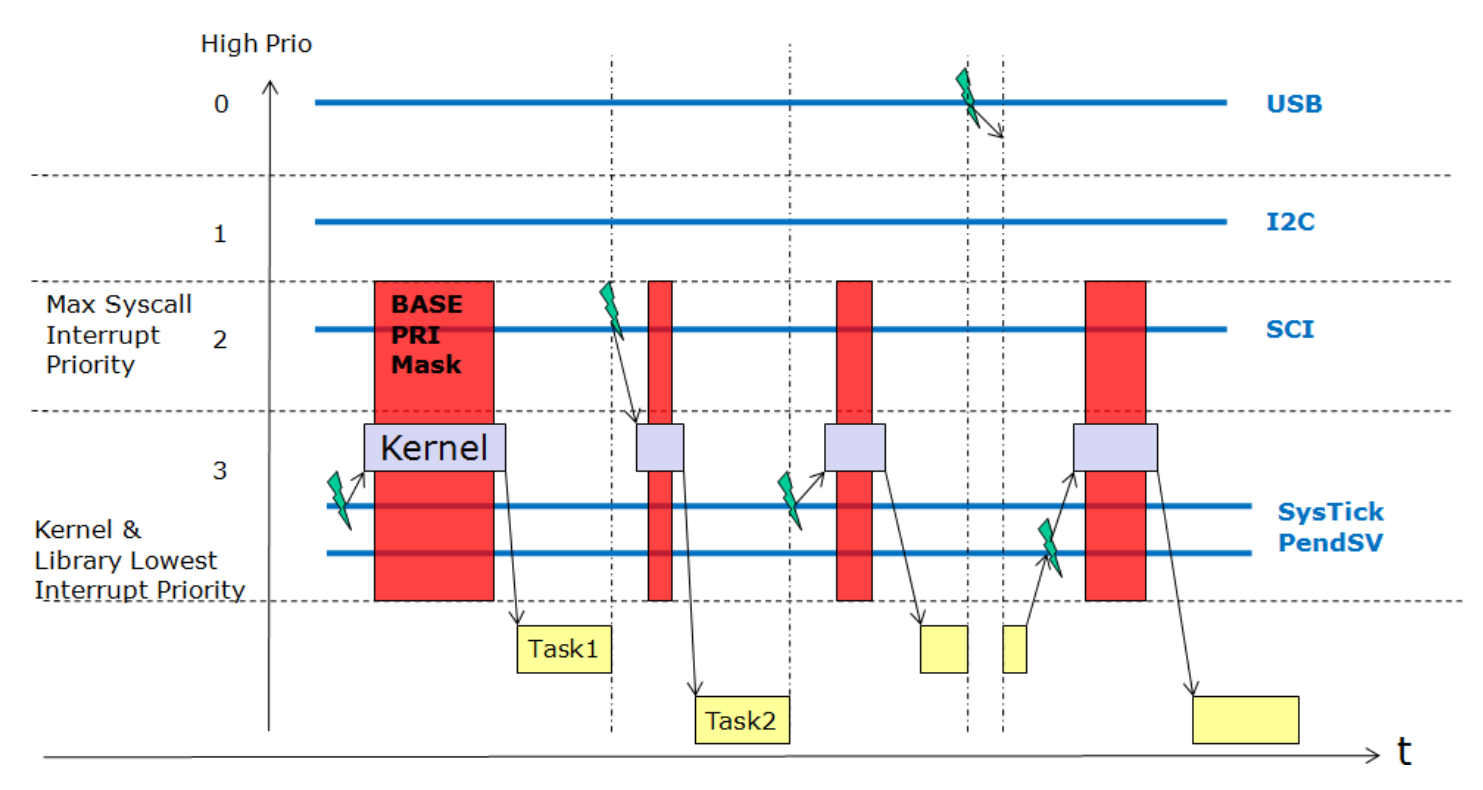
\includegraphics[width=0.6\linewidth,left]{img/ARM_Interrupt_Priorities.PNG}
							Aus irgend einem Grund ist es wichtig, dass Systick und PendSV mit der geringsten Dringlichkeit agieren. Die applikations taskshaben virtuell
							auch die geringste priorität(ok demfall?). Daher können diese auch jeder Zeit von jedem Interrupt unterbrochen werden (isch glaub guet demfall).
							Wen der Interrupt für den Kernel ist (SysTick oder PendSV -> hä?) dann wird der kernel allen interrupts sofort den max Syscall Interrupt Priority zuweisen.
							Dann wird der Kernel nicht von den weniger stark priorisierten Interrupts belästigt( aber welche interrupts erhalten denn jetzt diese Prio?). Zusätzlich dazu 
							vereinfacht dann dies die reentrancy des Kernelcodes. Wieso? sobald der Kernel die BASEPRI interrupt Blockierung aktiviert hat,  ist der Kernel von Aufrufen durch fromISR()
							und anderen RTOS API aufrufen geschützt (hä? was? ok...). Allerdings heisst das aber, dass Interrupt mit einer höheren Prio als der max Syscall Interrupt Priority den Kernel 
							unterbrechen können (also die Ausführung dessen Codes) und nicht von dessen Verzögerung beeinträchtigt sind. Warum auch immer bedeutet das, dass solche interrupts nicht  
							einfach alle RTOS API funktionen verwenden können.... nüt hani verstande.
				\end{description}
			\subsection{Tasks}	
				\begin{description}
					\item[$\bullet$ Priority-based Preemptive Scheduling]
						FreeRTOS kann für zwei verschiedene scheduling modes konfiguriert werden. Dies wird vom konfigurationsmakro config\_USE\_PREEMPTION 
						kontrolliert?
						\begin{itemize}
							\item Preemptive Scheduling: Der Scheduler hat die Kontrolle über die CPU und kann laufende Tasks abbrechen.
							\item Cooperative Scheduling: Der Task behält kontrolle über die CPU bis er diese wieder an den Scheduler zurück gibt.
						\end{itemize}
						FreeRTOS verwendet ein Prioritäten basierendes Preemptive Scheduling. Das bedeutet, dass der Scheduler immer den ready task mit der 
						höchsten Priorität "laufen" lässt. Es muss aufgepasst werden, dass die tasks mit tiefer Priority auch zum zug kommen (ja und wie macht man 
						das?).
						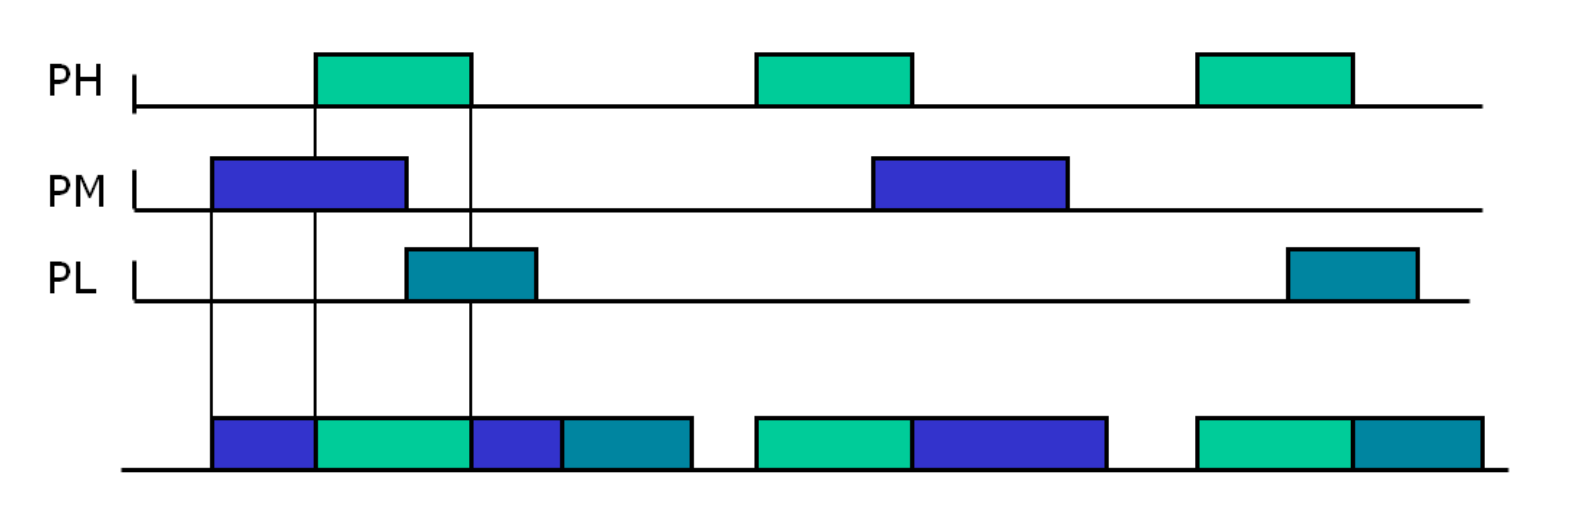
\includegraphics[width=0.6\linewidth,left]{img/Prioritybased_preemptive_scheduling.PNG}
						Jeder Task hat eine Priorität (0 bis config-MAX\_PRIORITIES - 1). Das Makro config-MAX\_PRIORITIES ist definiert in FreeRTOSConfig.h.
						Falls mehrere Tasks mit gleicher Priorität zur gleichen Zeit gelöst werden sollen, wird der Scheduler time-slicing andwenden (dies wird im file
						configUSE\_TIME\_SLICING kontrolliert) und allen Tasks
						gleich viel Rechenzeit gewährleisten.
					\item[$\bullet$ Task States]
						In FreeRTOS kan jeder der tasks in einem der folgenden Zustände sein:
							\begin{itemize}
								\item Running: Der Task wird auf der CPU ausgeführt. Es kann nur ein Task auf einmal ausgeführt werden.
								\item Suspended: Der Task muss nichts ausführen, der task schläft.
								\item Ready: Der Task ist bereit für die Ausführung (nicht suspended oder blocked), wurde noch nicht vom Scheduler zum Ausführen gebracht
								\item Blocked: Der Task ist blockiert, wartet also auf ein Objekt oder ein Event.
							\end{itemize}
							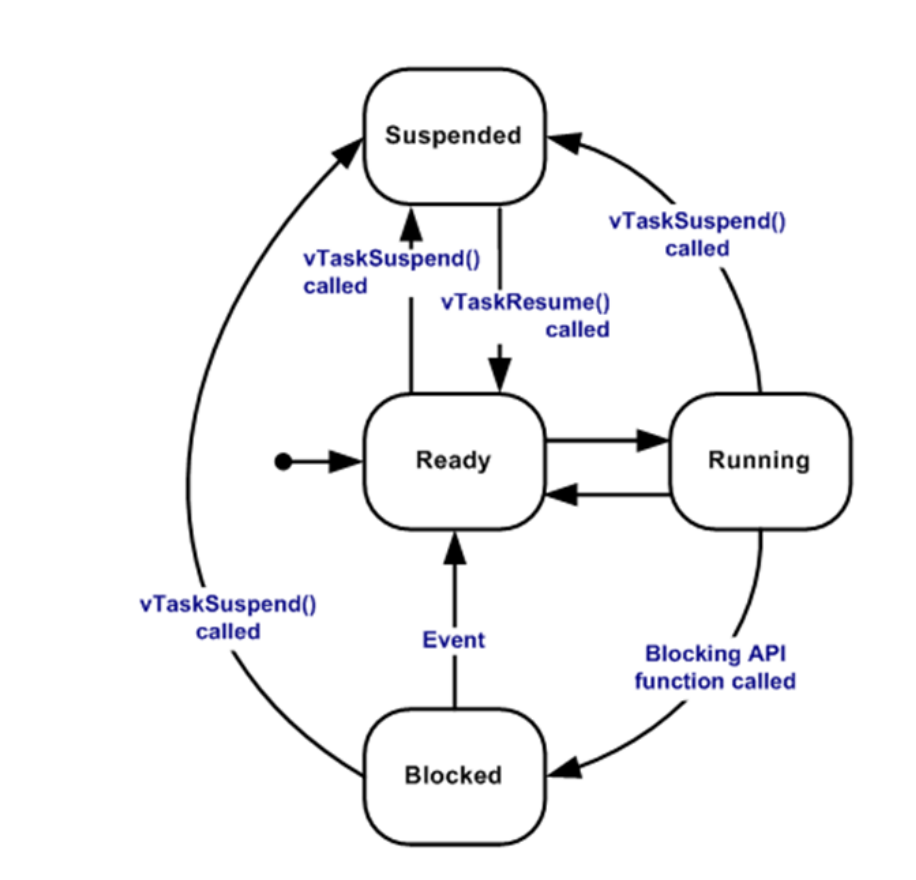
\includegraphics[width=0.6\linewidth,left]{img/Task_State_transistions.PNG}
					\item[$\bullet$ Time Slicing]  
						Falls configUSE\_TIME\_SLICING nicht definiert ist oder auf 1 gesetzt ist, dann wird FreeRTOS standardmässig time slicing zwischen tasks verwenden. 
						RTOS wird also den ready Task mit der höchsten Priorität starten. CPU Zeit wird zwischen den ready Tasks mit gleicher priorität aufgeteilt(steht irgendwas 
						mit time of the tick interrupt, versteh isch nisch oida).Falls configUSE\_TIME\_SLICING 0 sein sollte, dann wird RTOS beim auftreten des TickInterrupts nicht zu einem anderen ready task mit der 
						selben Priorität wechseln.
					\item[$\bullet$ IDLE Task]
						\begin{itemize}
							\item IDLE Task wird von vTaskStartScheduler() erstellt.
							\item Wird mit Hilfe von tskIDLE\_PRIORITY und configMINIMAL\_STACK\_SIZE erstellt.
							\item Läuft immer wenn kein anderer Task Läuft.
							\item Falls in einer Anwendung vTaskDelete() verwendet wurde, räumt IDLE Task den Speicher auf.
								Daher sollte man schauen dass der IDLE Task immer Rechenzeit erhält (nicht ausgehungert wird).
							\item Ruft IDLE Hook auf.
						\end{itemize}
						\begin{lstlisting}
static void prvIdleTask ( void * pvParameters ) {
	for (;;) {
		RemoveDeletedTasksFromList () ;
		if (! configUSE_PREEMPTION ) {
			taskYIELD () ;
		} else if ( configIDLE_SHOULD_YIELD ) {
			if ( NofReadyTasks ( tskIDLE_PRIORITY ) >1) {
				taskYIELD () ;
			}
		}
		IdleHook () ;
	} /* for */
}
						\end{lstlisting} 
						configIDLE\_SHOULD\_YIELD bestimmt beim einem preemtiven Scheduler ob
						der IDLE Task gleich die Kontrolle an einen Task im Ready Zustand abgeben
						soll, oder ob er auf die n"achste Unterbrechung (Preemption) warten soll. Hierzu
						wird ein taskYIELD() verwendet, welches einen Kontextswitch veranlasst.
					\item[$\bullet$ Blinky Task]
					Beispiel BLinkyTask erstellen. Wird entweder im main() oder innerhalb eines anderen Tasks erstellt.
						\begin{lstlisting}
BaseType_t res ;
TaskHandle_t taskHndl ;
res = xTaskCreate ( BlinkyTask , /* function */
	" Blinky ", /* Kernel awareness name */
	500/ sizeof ( StackType_t ) , /* stack */
	( void *) NULL , /* task parameter */
	tskIDLE_PRIORITY +1 , /* priority */
	& taskHndl /* handle */
	);
if ( res != pdPASS ) { /* error handling here */ }
						\end{lstlisting}  
							\begin{itemize}
								\item xTaskCreate() wird der Task erstellt
								\item Als erstes Argument wird der Name (oder besser: Funktionszeiger) (BlinkyTask) der Task Funktion ubergeben.								
								\item Danach werden ein String mit dem Namen (Blinky) f"ur den Debugger und der Task Awareness.							
								\item 500/sizeof(StackType\_t) gibt Anzahl Bytes auf Stack. Als alternative könnte man auch configMINIMAL\_STACK\_SIZE verwenden,
								\item $( void *) NULL$ ist ein optionaler Input Parameter. dieser Zeiger wird dem Task als Argument
								 "ubergeben, kann aber auch mit NULL gesetzt werden.Es ist zu beachten, dass das Objekt auf das der Zeiger zeigt zur Taskausfuhrungszeit auch ¨
								 noch existiert, das heisst z.B. auf eine globale Variable zeigt.
								\item tskIDLE PRIORITY gibt üblicherweise die Priorität des Tasks an, hier also 0.  Optional kann auch ein Task Handle
								angegeben werden (call-by-reference), d.h. wo der Handle gespeichert werden
								soll.
								\item xTaskCreate() gibt einen Fehler Code vom Typ BaseType\_t zrur"uck. Falls xTaskCreate() ein pdPASS zur"uckgibt hat es funktioniert, ansonsten ist ein 
								Fehler aufgetreten, z.B. war nicht gen"ugend Speicher vorhanden.
							\end{itemize}
							Der Task selber Sieht wie eine normale Funktion aus:
						\begin{lstlisting}
static void BlinkyTask ( void * pvParameters ) {
	( void ) pvParameters ; /* not used */
	for (;;) {
		LED_Neg () ;
	}
}
						\end{lstlisting}  
						Der Task l"auft normalerweise in einer Endlosschleife (ausser er l"oscht sich selbst). Der Task hat kein Return da er nirgends zurückkehren kann.
						Man sieht auch den Task Parameter (void Zeiger) welcher beim einstellen angegben wurde. Bei nicht-nutzung kann der Parameter auch auf coid gecastet werden, 
						damit der Compiler keine Warnung ausgibt.
						Im oben Dargestellten Code wird die LED so schnell wie m"oglich negiert. Der Task verwenet die ganze Rechenzeit. Dies ist unbefriedigend, man sollt dem
						Scheduler Rechenzeit zur"uck geben.
						\begin{lstlisting}
static void BlinkyTask ( void * pvParameters ) {
	for (;;) {
		LED_Neg () ;
		vTaskDelay ( pdMS_TO_TICKS (50) ) ;
	}
}
						\end{lstlisting}  
						\begin{itemize}
							\item vTaskDelay() gibt Rechenzeit zurück, da ja sonst die armen Tasks mit niedriger Prio hungern müssen.
							\item pdMS\_TO\_TICKS berechnet ben"otigte Ticks.
						\end{itemize}
						\begin{lstlisting}
/* Converts a time in milliseconds to a time in ticks . This macro
can be overridden by a macro of the same name defined in
FreeRTOSConfig .h in case the definition here is not suitable for
your application . */
#ifndef pdMS_TO_TICKS
	#define pdMS_TO_TICKS ( xTimeInMs ) \
		(( TickType_t ) ((( TickType_t ) ( xTimeInMs ) * ( TickType_t )
			configTICK_RATE_HZ ) / ( TickType_t ) 1000) )
#endif
						\end{lstlisting}  
						\begin{itemize}
							\item configTICK\_RATE\_HZ ist 1000 (1 ms), dann ergibt pdMS\_TO\_TICKS(50) die
							Anzahl von 50 Ticks.						
							\item configTICK\_RATE\_HZ ist 100 (10 ms), dann ergibt pdMS\_TO\_TICKS(50) die
							Anzahl von 5 Ticks.
							\item configTICK\_RATE\_HZ ist 100 (10 ms), dann ergibt pdMS\_TO\_TICKS(15) die
							Anzahl von 1 Tick. Beachte dass die Division ganzzahlig ist.
						\end{itemize}
						Das Macro pdMS TO TICKS kann auch anwendungsspezifisch "uberschrieben werden
						Dies ist z.B. n"otig, falls man eine Tick Frequenz h"oher als 1 ms verwenden
						m"ochte.Das vTaskDelay() wartet die angegebene Anzahl Ticks vom Zeitpunkt des
						Aufrufs. F"ur das folgende Beispiel bedeutet dies, dass der Task nicht mit 
						einer fixen Frequenz l"auft, sondern je nachdem wie viel Zeit im ’do something’
						verbraucht wird:
						\begin{lstlisting}
static void MyTask ( void * pvParameters ) {
	for (;;) {
		/* do something here */
	vTaskDelay ( pdMS_TO_TICKS (50) );
	}
}
						\end{lstlisting}  
						M"ochte man eine fixe Frequenz erreichen, muss man vTaskDelayUntil()
						verwenden:
						\begin{lstlisting}
void vTaskDelayUntil ( TickType_t * pxPreviousWakeTime , const
	TickType_t xTimeIncrement );
						\end{lstlisting}  
						Hierbei ubergibt man als ersten by-reference Parameter einen Zeiger auf die ¨
						Zeit (Tick Count), bei der man zuletzt am Laufen war:
						\begin{lstlisting}
static void BlinkyTask ( void * pvParameters ) {
	TickType_t xLastWakeTime = xTaskGetTickCount () ;
	for (;;) {
		LED_Neg () ;
		vTaskDelayUntil (& xLastWakeTime , pdMS_TO_TICKS (50) ) ;
	}
}
						\end{lstlisting} 
						Den aktuellen Tick Z"ahler bekommt man mit xTaskGetTickCount(). Den
						Wert "ubergibt man dann als Zeiger. Damit weiss das Betriebssystem, wie lange
						vTaskDelayUntil() effektiv warten soll. Der Wert des Z"ahlers ist dann bei der
						R"uckkehr von vTaskDelayUntil() auf den neuen Wert angepasst, muss ihn also
						nicht nochmals setzen. Damit wird eine konstannte Frequenz des Tasks erreicht,
						unabh"angig der Ausfuhrungszeit des Tasks.
					\item[$\bullet$ Task Control Ubersicht]
						Mit dem FreeRTOS Task Control API wird die Ausf"uhrung der Tasks beeinflusst:
					\begin{itemize}
						\item Task verz"ogern: vTaskDelay(), vTaskDelayUntil()
						\item Prio zur Laufzeit "andern: uxTaskPriorityGet(), vTaskPrioritySet()
						\item Task anhalten und weiterfahren lassen: vTaskSuspend(),
						vTaskResume(), vTaskResumeFromISR()	
						\item vTaskPrioritySet: Beim Erstellen eines Tasks wird schon eine Priorit"at zugewiesen. Man kann zur
						Laufzeit die Priorit"at von Tasks "andern, um zum Beispiel auf eine ge"anderte
						Auslastung zu reagieren. Generell sollte man dies aber sehr sorgf"altig planen,
						da eine dynamische Anderung des Systems die Komplexit"at erh"oht und zu unerwunschten Nebeneffekten f"uhren kann. Um die Priorit"at eines Tasks zu "andern
						braucht man den Task Handle oder NULL fur den aufrufenden Task. Auch sollte ¨
						die Funktion nur von einem Task Kontext benutzt werden
						\begin{lstlisting}
void vTaskPrioritySet ( TaskHandle_t pxTask , unsigned portBASE_TYPE
	uxNewPriority );
						\end{lstlisting}
						Nachfolgend ein Beispiel, bei dem die Priorit¨at eines Tasks um 1 erh¨oht wird.	
						\begin{lstlisting}
xTaskCreate ( vTaskCode , " MyTask ", configMINIMAL_STACK_SIZE , NULL ,
	tskIDLE_PRIORITY , & xHandle );
...
vTaskPrioritySet ( xHandle , tskIDLE_PRIORITY +1) ;
						\end{lstlisting}			
					\end{itemize} 
				\end{description}
			\subsection{Kernel Control}
				Die Kernel Control API ermöglicht es einem den Kernel zu Kontrollieren.
				\begin{itemize}
					\item Starten und Beenden des Kernels: vTaskStartScheduler(), vTaskEndScheduler() 						
					\item Kernel Task Switching und anhalten und wieder einschalten: vTaskSuspendAll(), vTaskResumeAll()
					\item Kontrolle an ready Task abgeben: taskYIELD()
				\end{itemize}
				\begin{description}
					\item[$\bullet$ vTaskStartScheduler]
						Startet den Scheduler: 
						\begin{lstlisting}
void vTaskStartScheduler ( void );
						\end{lstlisting}  
						\begin{itemize}
							\item Bewirkt Wechsel vom Init zum Running state.						
							\item Erstellt den IDLE task mit config\_MINIMAL\_STACK\_SIZE und tskIDLE\_PRIORITY.
							      Falls SoftwareTimer aktiviert sind wird auch ein daemon timer aktiviert (was au immer das si sött...)
							\item Der ready task mit der höchsten Priorität wird gestartet ( bin mit nicht sicher ob das jetzt von den Softw timern abhängt, aber denke nicht)
							\item Kehrt nicht zur"uck bis vTaskEndScheduler()  aufgerufen wird.
							\item Meistens werden zuerst alle Tasks erstellt und dann wird vTaskStartScheduler() aufgerufen. 
						\end{itemize}
					\item[$\bullet$ vTaskEndtScheduler]
						\begin{lstlisting}
void vTaskEndScheduler ( void );
						\end{lstlisting} 
						\begin{itemize}
							\item Beendet den Kernel						
							\item Springt dort zur"uck wo vTaskStartScheduler() aufgerufen wurde.
							\item Ben"otigt setjmp(), lingjmp() welche nicht f"ur jeden FreeRTOS port implementiert sind.
								  Der MCUOnEclipse FreeRTOS port hat dies f"ur alle architekturen implementiert.
						\end{itemize} 	
					\item[$\bullet$ vTaskSuspendAll]
						\begin{lstlisting}
							void vTaskSuspendAll ( void );
						\end{lstlisting}  
						\begin{itemize}
							\item Erzwingt den Wechsel vom aktiven in den suspended Zustand
							\item Nach dem Aufruf dieser Funktion wird kein Kontext switch vorkommen bis xTaskResumeAll() aufgerufen wurde.					
						\end{itemize} 
					\item[$\bullet$ xTaskResumeAll]
						\begin{itemize}
							\item Ist das Gegenteil von SuspendAll-Y bringt den Kernel zurück in den Aktiven Zustand.
							\item Der R"uckgabewert der Funktino ist pdFALSE falls kein bzw pdTRUE falls ein kontext switch mit dem API aufruf stattgefunden hat.
							\item Ist pdFalse falls kernel noch im suspended state ist.					
						\end{itemize} 
					\item[$\bullet$ taskDISABLE ENABLE\_Interrupts]
					Codebeispiel:
						\begin{lstlisting}
void taskENTER_CRITICAL ( void ) ;
void taskEXIT_CRITICAL ( void );
void vPortEnterCritical ( void ) {
	portDISABLE_INTERRUPTS () ;
	uxCriticalNesting ++;
}
void vPortExitCritical ( void ) {
	uxCriticalNesting - -;
	if ( uxCriticalNesting == 0) {
		portENABLE_INTERRUPTS () ;
}
}
						\end{lstlisting} 						
						\begin{itemize}
							\item taskENTER CRITCAL() und taskEXIT CRITCAL() werden um im Kernel die task Critical section zu machen. 
							\item Critical Section deaktiviert die Interrupts aber nur auf Kernel level.
							\item Die Implementation verwendet einen counter welcher das nesting kritischer makros erlaubt.
							\item Es gibt Ports die Interrupts immer Erlauben wenn der Counter null erreicht. Auch wenn 
								  taskENTER CRITCAL() verwendet wurde (alte was)
							\item Keine anderen FreeRTOS API Funktionen innerhalb eines kritischen bereichs eines Tasks aufrufen (hä).
						\end{itemize}
					\item[$\bullet$ taskYELD]
					Codebeispiel: 
						\begin{lstlisting}
#define taskYIELD () portYIELD ()
#define portYIELD () vPortYieldFromISR ()
void vPortYieldFromISR ( void ) {
	/* Set a PendSV to request a context switch . */
	*( portNVIC_INT_CTRL ) = portNVIC_PENDSVSET_BIT ;
	/* Barriers are normally not required but do ensure the code is
		completely within the specified behavior for the architecture
		. */
	__asm volatile (" dsb ");
	__asm volatile (" isb ");
}
						\end{lstlisting}
						\begin{itemize}
							\item task YIELD() ist typischerweise als makro implementiert. 
							\item damit kann ein task einen Kontext switch verlangen.
							\item im kooperativen RTOSmodus kann so ein task kontrolle zurück an den kernel geben, der scheduler wird dann
								  den nächst höher priorisierten Task (h"a)
						\end{itemize}
					\end{description}
			\subsection{RTOS Visualisierungen}
				Hilfsmittel zur Überwachung des Systemzustandes.
					\begin{description}				
						\item[$\bullet$ Eclipse Plugins]
							Viele Eclipse IDE Distributionen wie etwa MCUXpresse haben spezielle Plugins und Views. Gewisse Erweiterungen erlauben
							sogar ein Debugging auf Taskebene. Die Meisten Views sind Stop Mode views. 
						\item[$\bullet$ Task List View]
							 Das Bild zeigt die Liste mit den Tasks. Damit diese Informationen verfügbar sind, muss ein \#define im FreeRTOSConfig.h 
							 eingeschaltet werden.
							 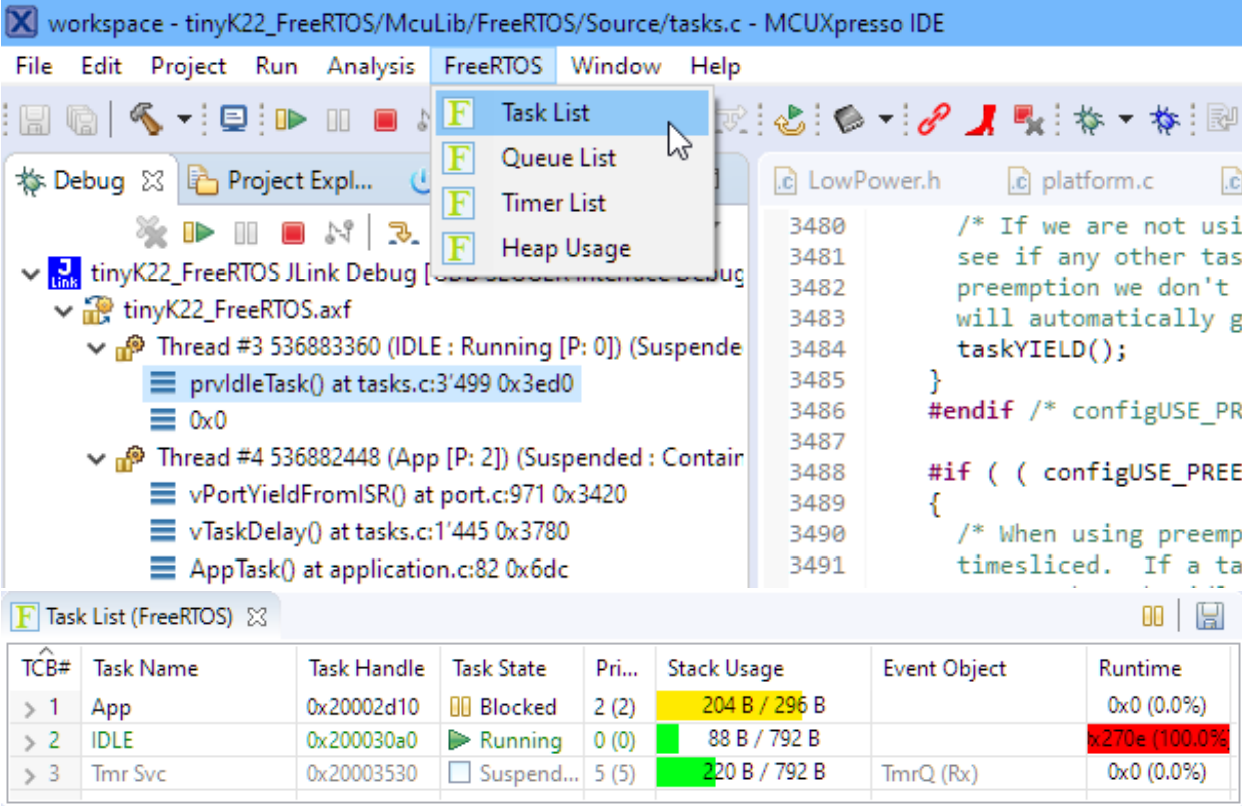
\includegraphics[width=0.6\linewidth,left]{img/Queue_List_view.PNG}
							 \begin{itemize}
								 \item Einschalten mit configUSE\_TRACE\_FACILITY
								 \item Informationen "uber Tasks: TCB (Task Control Block), Namen, Handle
								 \item Task Zustand, Basis Priorit"at und aktuelle Priorit"at
								 \item Stack Benutzung
								 \item Event Objekte: worauf der Task wartet/blockiert ist
								 \item Runtime: Wieviel Prozent der Rechenzeit benutzt
							 \end{itemize}
						\item[$\bullet$ Queue List View]	
							Mit dieser Ansicht k"onnen die aktuellen Queues im System angezeigt werden
							. Da in FreeRTOS sowohl Semaphore und Mutex mit Queues
							realisiert sind, dient diese Anzeige auch daf"ur. Da die Queues in FreeRTOS 
							ohne Namen erstellt werden, sollten diese zur Laufzeit mit einem Namen in der
							Registry versehen werden
							\begin{itemize}
								\item Anzeigen der Queues, inklusive Semaphore und Mutex
								\item Queue Name muss mit vQueueAddToRegistry() registriert werden
								\item configQUEUE REGISTRY SIZE in FreeRTOSConfig.h
							\end{itemize}
							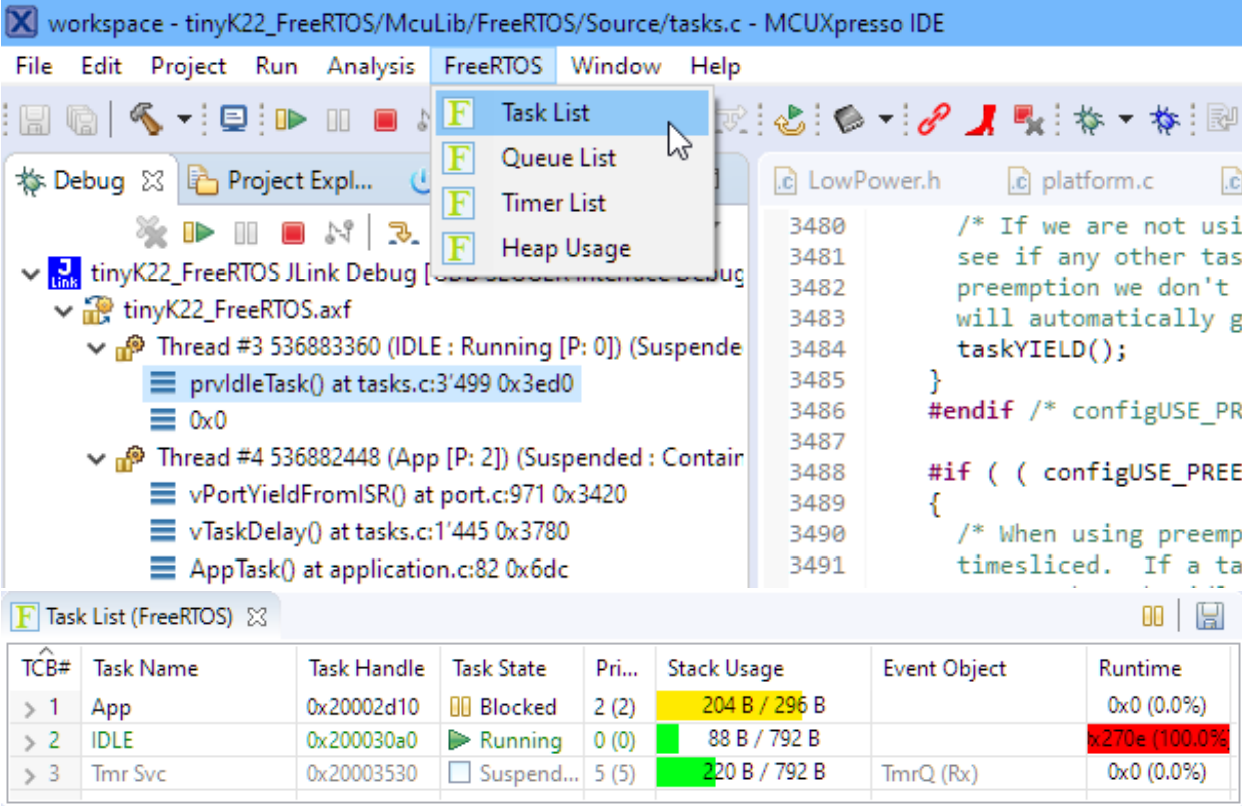
\includegraphics[width=0.6\linewidth,left]{img/Queue_List_view.PNG}
							Nachfolgend ein Beispiel, wie man die Registry auf 10 Eintr¨age einstellt:
							\begin{lstlisting}
#define configQUEUE_REGISTRY_SIZE 10
							\end{lstlisting}
							Untenstehendes Beispiel zeigt, wie man nach dem Erstellen einer Queue ihr
							einen Namen gibt, damit man diese im Debugger ansehen kann:
							\begin{lstlisting}
static xQueueHandle SQUEUE_Queue ;
Queue = xQueueCreate ( SQUEUE_LENGTH , SQUEUE_ITEM_SIZE );
if ( Queue == NULL ) {
	for (;;) {} /* out of memory ? */
}
vQueueAddToRegistry ( Queue , " ShellQueue ");
							\end{lstlisting}
							Sollten die Pl"atze nicht ausreichen, kann man jederzeit einen Namen mit
							vQueueUnregisterQueue() wieder austragen. Dies geschieht auch wenn man
							die Queue l"oscht.
						\item[$\bullet$ Segger Real Time Transfer] 
						Die bisherigen Möglichkeit verwenden den Debugger, um Daten über das Betriebssystem anzuzeigen. 
						Eine andere M"oglichkeit ist es w"ahrend dem Laufen der Anwendung die Daten 2uber einen Kommunikatinoskanal zu "ubertragen.
						Ein Weg dazu ist die Verwendung von SEGGER RTT:
						\begin{itemize}
							\item Bidirektionale Kommunikation "uber Debug Schnittstelle
							\item Ben"otigt SEGGER J-Link Hardware oder Debug Schnittstelle (z.B OpenSDA)
							\item Kleiner Speicherbedarf: 500 Bytes Flash, 50 RAM pro Kanal
							\item Spezielle Viewer oder Telnet (Port 19021) (McuOnEclipse nachlesen)
						\end{itemize}
						Mittels dem RTT Protokoll k"onnen nun Daten w"ahrend dem Betrieb gesendet werden und z.B vom SystemViewern dargestellt werden 
						\item[$\bullet$ FreeRTOS Trace Hooks]
						Damit RTOS Daten senden Kann, muss es zuerst instrumentiert werden. Dies geschieht durch Hooks, wie im folgenden Bsp:
						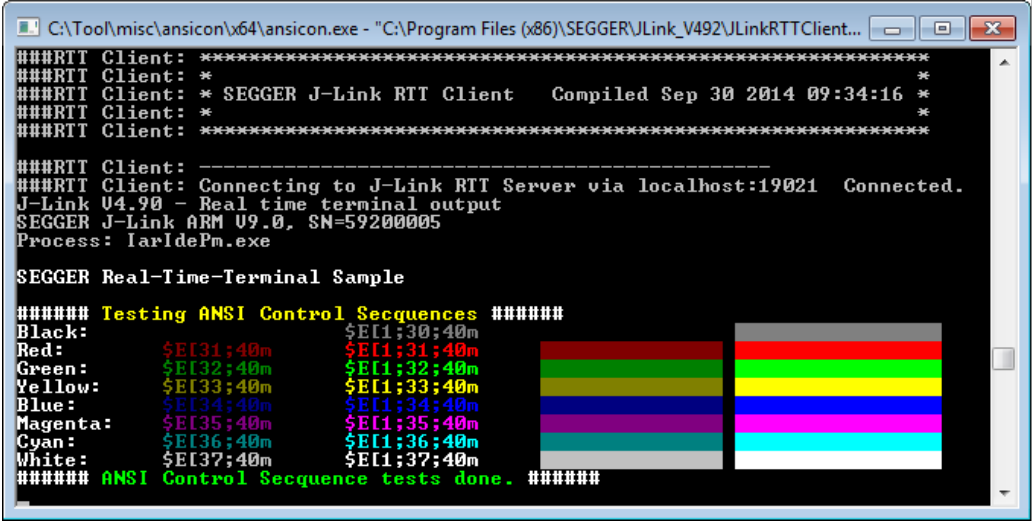
\includegraphics[width=0.6\linewidth,left]{img/Segger_RTT_Client.PNG}	 
						\begin{lstlisting}
#ifndef traceTASK_SWITCHED_OUT
	/* Called before a task has been selected to run . pxCurrentTCB
		holds a pointer
	to the task control block of the task being switched out . */
	#define traceTASK_SWITCHED_OUT ()
#endif
						\end{lstlisting}
						Diese Hooks werden dann verwendet, um Daten zu senden und aufzuzeichnen
						\begin{itemize}
							\item Trace Hooks im Kernel (Instrumentierung): Task erstellen, Kontext switch, 
							\item Kernel meldet an strategischen Stellen Aktivität
							\item Einschalten mit configUSE\_TRACE\_HOOKS
								  \begin{itemize}
									\item Eigenes Aufzeichnen und Tracing
									\item Percepio FreeRTOS + Trace
									\item Segger System Viewer
								  \end{itemize}	
						\end{itemize}
						\item[$\bullet$ Segger System Viewer]
							Mit so einem Viewer kann der momentane Zustand des Systems und auch der Ablauf "uber die Zeit betrachtet werden.
						\item[$\bullet$ Percepio Tracealizer]
		 
					\end{description}
				\subsection{Reentrancy}
					\begin{description}
						\item[$\bullet$ Gemeinsamer Code:]
							Im Softwareengeneering wird der Code oftmals einem Refactoring unterzogen. Ein Teil dieses Refactoring ist es 
							teile des Codes in gemeinsame Subroutinen zusammenzufassen. Jetzt kann es vorkommen dass genaud dieser Code vorkommen
							Hauptprogramm und von der ISR genutzt wird.
							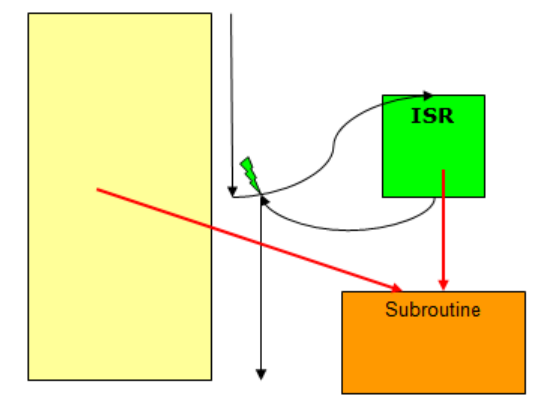
\includegraphics[width=0.6\linewidth,left]{img/Common_Subroutines.PNG}
							\item[$\bullet$ Gemeinsame Daten]
							\item[$\bullet$ Reentrancy] 
								Mit reentrancy bezeichnet man das Wiedereintreten in eine Subroutine. Das Problem dabei ist, dass unter Umständen
								Zwei Programme auf die Gleiche Variable zugreiffen und diese dann verändern. Das würde zu falschen Resultaten führen.
								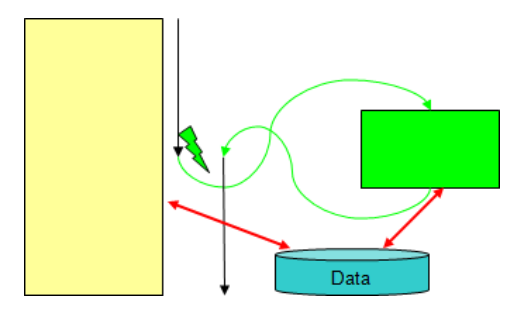
\includegraphics[width=0.6\linewidth,left]{img/Common_Data.PNG}
								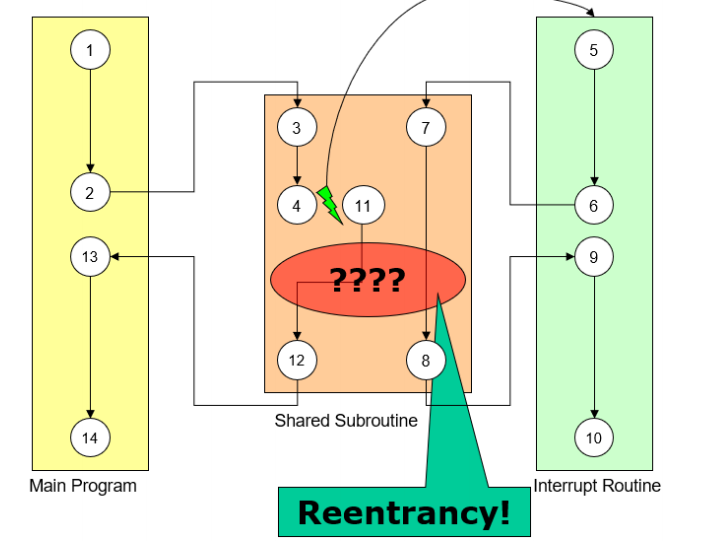
\includegraphics[width=0.6\linewidth,left]{img/Wieder_eintreten_gemeinsame_Subroutine.PNG}  
								Da jeder Zeit ein Interrupt auftreten kann,  muss jede Soubroutine reentrant sein (was heisst das? Wieso).
								Im Unten dargestellten Beispiel wird eine Variable hochgezählt, immer wenn einer Von zwei Tastern gedrückt wird.
								\begin{lstlisting}
int cntr = 0;

void BtnA ( void ) {
	cntr ++;
	printf ("a: %d\r\n", cntr );
}

void BtnB ( void ) {
	cntr ++;
	printf ("b: %d\r\n", cntr );
}
								\end{lstlisting}
								Man erwartet jetzt eigentlich, das der Variablen wert immer um eins erhöht wird. Dies ist aber nicht der Fall.
								\begin{lstlisting}
	a: 1
	b: 2
	a: 3
	b: 4
	a: 4
								\end{lstlisting}
								Der Grund dafür ist, dass das Erhöhen des Z"ahlers mit einer Load-Increment-Store Sequenz gemacht wird. Hierbei kann 
								es passieren, dass ein Interrupt die Sequenz unterbricht und zu einem Falschen Resultat führt.
								\begin{lstlisting}
ld cntr , R0 (3)
inc R0 (4)
			ld cntr , R0 (3)
			inc R0 (4)
			st R0 , cntr (4)
			print cntr (4)
st R0 , cntr (4)
prinf cntr (4)
								\end{lstlisting}
								Einfach gesagt; Die Taste wird gedrückt, es soll eine 4 gespeichert werden. Es werden 4 Assembly Schritte dafür benötigt.
								Ein Interrupt unterbricht aber beim zweiten Schritt, da die Taste ein Zweites Mal gedrückt wurde. Jetzt wird 3 um eins erhöht und 4 wird abgespeichert.
								Dann geht der Code zur"uck und speichert nochmals die 4 die vor dem unterbruch erzeugt wurde. 
							\item[$\bullet$ Disable and Enable Interrupts] 	
								Diese Problem wird durch das Unterbrechen von Interrupts generiert. Man kann dieses Problem also umgehen, indem man
								das Unterbrechen von Interrupts verhindert. Die Sprache C hat keine Interrupt Unterst"utzung, man muss dies daher mit
								Makros umsetzen. Bsp f"ur Cortex.
								\begin{lstlisting}
#define DISABLE_INTERRUPTS { __asm volatile (" cpsid i") ;}
#define ENABLE_INTERRUPTS { __asm volatile (" cpsie i") ;}
								\end{lstlisting}
								Damit kann man folgende Subroutinen reentrant machen.
								\begin{lstlisting}
#define DISABLE_INTERRUPTS { __asm volatile (" cpsid i") ;}
#define ENABLE_INTERRUPTS { __asm volatile (" cpsie i") ;}
int cntr = 0; /* number of people in the room */

void Inc ( void ) {
	DISABLE_INTERRUPTS ;
	cntr ++;
	ENABLE_INTERRUPTS ;
}

void Dec ( void ) {
	DISABLE_INTERRUPTS ;
	cntr - -;
	ENABLE_INTERRUPTS ;
}
								\end{lstlisting}
								Dies f"uhrt zu folgender verbesserter Version
								\begin{lstlisting}
void Inc ( void ) {
	DISABLE_INTERRUPTS ;
	cntr ++;
	ENABLE_INTERRUPTS ;
}
								\end{lstlisting}
								\begin{lstlisting}
void doCounting ( void ) {
	DISABLE_INTERRUPTS ;
	if ( cntr <100) {
	Inc () ;
	}
	print ( cntr );
	ENABLE_INTERRUPTS ;
}
								\end{lstlisting}
								Problem hierbei ist, dass alle Interrupts eher lange ausgeschaltet sind. Dies f"uhrt zu einer grossen Interrupt Latenz.
								Zudem werden in der Funktion Inc() die Interrupts wieder eingeschaltet.
								Eine weiter Optimierung könnte so Aussehen.
								\begin{lstlisting}
void Inc ( void ) {
	DISABLE_INTERRUPTS ;
	cntr ++;
	ENABLE_INTERRUPTS ;
}
								\end{lstlisting}
								Die Variable cntr w"urde wie folgt benutzt:
								\begin{lstlisting}
void doCounting ( void ) {
	DISABLE_INTERRUPTS ;
	bool isLess = cntr <100;
	ENABLE_INTERRUPTS ;
	if ( isLess ) {
		Inc () ;
	}
	DISABLE_INTERRUPTS ;
	print ( cntr );
	ENABLE_INTERRUPTS ;
}
								\end{lstlisting}
								Diese Variante verschlimmert alles. Die Variable ist zwar geschützt, aber falls die Ausgabe des Z"ahlers zusammenh"angen soll, wird dies nicht erreicht.
								Das Heisst wir m"ussen uns etwas anderes "uberlegen.
							\item[$\bullet$ Disable and Enable Interrupts]
					Problem beim ein und ausschalten von interrupts $\rightarrow$ es können unbeabsichtigt interrupts wider eingeschaltet werden.
								\begin{lstlisting}
void Inc ( void ) {
	DISABLE_INTERRUPTS ;
	cntr ++;
	ENABLE_INTERRUPTS ;
}

void main ( void ) {
	/* interrupts are disabled , we will enable them later */
	Inc () ;
	/* Upps ! interrupts are suddenly enabled ! */
}
								\end{lstlisting}
								Es scheint also irgendwie noch sinnvol ztu sein zu Wissen ob beim verlassen der Critical Section(Wasch di critical section?)
								die Interrupts schon ausgeschaltet waren oder nicht. Dazu kann man ja den Zustand in einer lokalen Variable speichern.
								\begin{lstlisting}
#define CriticalVariable () \
	uint8_t cpuSR /* variable to store current status */
								\end{lstlisting}
								Hiermit kann man nun per Inline Assembler den Zustand in dieser Variable speichern.
								\begin{lstlisting}
#define EnterCritical () \
	do { \
		__asm ( \
			" mrs r0 , PRIMASK \n"\
			" cpsid i \n"\
			" strb r0 , cpuSR \n"\
	); \
} while (0)
								\end{lstlisting}
								Beim Verlassen der Critical Section wird dann der vorherige Zustand hergestellt:
								\begin{lstlisting}
#define ExitCritical () \
	do { \
		__asm ( \
		" ldrb r0 , cpuSR \n"\
		" msr PRIMASK ,r0 \n"\
	); \
} while (0)
								\end{lstlisting}
								Hiermit kann man eine Critical Sectino nun auch veschachtelt realisieren:
								\begin{lstlisting}
void Inc ( void ) {
	McuCriticalSection_CriticalVariable () ;

	McuCriticalSection_EnterCritical () ;
	cntr ++;
	McuCriticalSection_ExitCritical () ;
}
void doCounting ( void ) {
	McuCriticalSection_CriticalVariable () ;
	
	McuCriticalSection_EnterCritical ;
	Inc () ;
	McuCriticalSection_ExitCritical ;
}
								\end{lstlisting}
								Damit w"are das Problem gel"ost.
					\end{description}
				\subsection{Heap Memory}
				FreeRTOS nutzt einen dynamischen Speicherbereich namens heap. Der Heap wird verwendet f"ur:
				\begin{itemize}
					\item Stack memory f"ur tasks
					\item RTOS interne Strukturen wie Task Control Block (TCB)
					\item Allozieren von Semaphoren, Mutex und Queues (was au immer die Begriff bedütend)
					\item Dynamische Speicherallozierung von programmen mit pvPortMalloc()
				\end{itemize}
				FreeRTOS kommt mit einer eigenen Heap implementation. Es unterst"utzt 5 verschiedene Speicher allozierungsarten(Schemes). Diese sind konfiguriert 
				von configFRTOS\_MEMORY\_SCHEME. Diese Sind implementiert in heap\_1.c, heap\_2.c etc. 
				Es kann immer nur eine Implementatino aktiv sein in einem Projekt.
				Die gr"osse des heap memory wird konfiguriert (in bytes) von configTOTAL\_HEAP\_SIZE.
				\begin{description}
					\item[$\bullet$ Heap Schemes]
					 Je nach Anwendung sollte eine passende Speicher allozierung verwendet werden. Da jede Allozierungsart ein eigenes file hat, 
					 ist es m"oglich eine eigene Allozierungsart zu implementieren.
					 \begin{itemize}
						\item Scheme 1: Speicher und Tasks k"onnen nur alloziert werden, aber nicht befreit(freed?). Funktioniert f"ur viele Anwendungen
							  wo Speicher zu beginn alloziert wird, aber nicht released. Das Schema ist deterministisch(timing kann garantiert werden)
							  , keine speicher Fragmentierung. (Und wieso)
						\item Scheme 2: Speicher bl"ocke k"onnen dealoziert werden. Freed Bl"ocke werden nicht gemerged. Dies kann zu Speicherfragmentierung f"uhren.
							  Es ist effizienter als das standard malloc() und free(), allerdings auch nicht deterministisch.
						\item Scheme 3: ist ein tread-safe wrapper ja fuck kein planen
						\item Scheme 4:Ist eigentlich das gleiche wie scheme 2, aber macht speicher merging und verhindert so speicherfragmentierung.
						\item Mach speicher block merging wie in scheme 4. Erm"oglicht das aufteilen des Heapspeichers in verschiedene Bl"ocke. Diese
							  Bl"ocke sind nicht angrenzend. vPortDefineHeapRegions() muss verwendet werden, um die speicher regionen zu definieren,
							  bevor speicher alloziert wird.?
					 \end{itemize}
					 \item[$\bullet$ Speicher Fragmentierung]
						 Mit scheme 2 ist es m"oglich Speicher zu fragmentieren, da die freien Speicherbl"ocke nicht zusammengef"uhrt werden. Selbst wenn genug
						 Speicher zur verf"ugung st"unde, allozieren eines neuen Blockes kann fehlschlagen, da die Bl"ocke nicht zusammengef"uhrt wurden. Je nachdem 
						 wie viele freie Speicherbl"ocke vorhanden sind, ist das System nicht deterministisch. Es braucht zeit, bis ein passender freier Block gefunden
						 wurde. Diese Scheme kann verwendet werden, wenn tasks, queues,semaphores,mutexes etc. gel"oscht werden sollen. Sollte nicht verwendet werden, wenn die
						 Anwendung zuf"allige oder dynamische allozierung bzw. deallozierung durchf"uhrt. Weil es eben zu Fragmentierung f"uhrt.
					\item[$\bullet$ Speicher f"ur die Anwendung]
						 FreeRTOS stellt folgende API zum allozieren und befreien von Speicher zur Verf"ugung(und die anzahl freier memory bytes).
						 \begin{itemize}
							\item pvPortMalloc() alloziert einen neuen Memory Block der gr"osse xWantedSize oder NULL wenn es nicht funktioniert hat.
							\item vPortFree() befreit einen zuvor allozierten Block. Da kein heap garbage collector vorhanden ist, muss die Anwendung nicht 
								  verwendete Speicherbl"ocke selbst freigeben.
							\item xPortGetFreeHeapSize() retourniert die totale anzahl freier bytes (inklusive fragmention? ok?). Diese methode kann nicht
								  zur Lokalisierung gr"osster Speicherbl"ocke verwendet werden(falls fragmentiert)ok?demfall....
						 \end{itemize}
						 \begin{lstlisting}
void * pvPortMalloc ( size_t xWantedSize );
void vPortFree ( void * pv );
size_t xPortGetFreeHeapSize ( void );
						\end{lstlisting}
						Bei dynamischer Speicher allozierung kann es immer vorkommen, dass der heap manager keine freien Speicherbl"ocke mehr findet.
						In diesem Fall ist der return Pointer NULL, und sollte "uberpruft werden. Der nachfolgend dargestellte Code allozierteinen neuen Speicherblock
						um einen String zu speichern. Der Block wird danach wieder befreit.
						 \begin{lstlisting}
void foo ( void ) {
	uint8_t * bufP ; /* pointer to buffer */
	bufP = ( uint8_t *) pvPortMalloc ( sizeof (" Hello ")) ;
	if ( bufP == NULL ) {
		for (;;) ; /* ups! Out of memory ? */
	}
	( void ) strcpy ( bufP , " Hello "); /* copy data */
	/* do something with data */
	vPortFree ( bufP ); /* release memory */
}
						\end{lstlisting}
				\end{description}

				\subsection{Hooks}
				Ermöglichen "uber Ereignisse (Hooks) informiert zu werden. (gleubs)
				\begin{description}
					\item[$\bullet$ "Ubersicht]
						Hooks sind in FreeRTOS synchrone Callbacks. Das System ruft "uber vordefinierte Namen Funktionen in der Anwendung auf.
						Diese Hooks sind optional, d.h. diese k"onnen, m"ussen aber nicht verwendet werden. Wenn man die 
						Hooks nicht ben"otigt, dann sollte man auf diese aus Performance-Gr"unden verzichten. Das Ein-und Ausschalten erfolgt "uber
						Makros im FreeRTOSConfig.h, wobei 0 den Hook ausschaltet. Es gibt folgende Hooks: 
						\begin{itemize}
							\item idle Hook
								Wird Aufgerufen, wenn das RTOS nichts zu tun hat. Dieser Hook wird of F"ur lowpoer Anwendungen ben"otigt.
							\item Tick Hook
								Wird aufgerufen f"ur jeden System Zeit Tick. Dieser kann als Timer Ersatz dienen.
							\item Malloc Failed Hook
								Wird aufgerufen wenn Speicherallozierung fehlschl"agt. Dieser Hook wird im Fehlerfall aufgerufen.
							\item Stack Overflow Hook
								Dieser Hook wird aufgerufen, wenn ein Stack"uberlauf festegestellt wird.
								Dieser Hook dient auch em Fehlerfall
						\end{itemize}
					\item[$\bullet$ Idle Hook]
						Folgendes Makro in FreeRTOSConfig.h kontrolliert den Idle Hook:
						\begin{lstlisting}
#define configUSE_IDLE_HOOK 1 /* 1: use Idle hook ; 0: no Idle
	hook */
#define configUSE_IDLE_HOOK_NAME vApplicationIdleHook
						\end{lstlisting}
							Mit dem ersten makro kann man den Hook ein oder ausschalten.Das zweite Makro definiert den namen der Funktion, welche aufgerufen wird.
							Der Idle Hook wird vom Idle Task bei jedem Schleifendurchlauf aufgerufen.
							Da der Idle Task nicht wirklich wartet, sondern dauernd die Schleife ausf"uhrt, kann es sein dass der Hook mehrfach und dauernd aufgerufen wird.
							Eine "ubliche Implementation ist es im Hook in den Low Power Modus zu gehen, bis ein interrupt den modus verl"asst:
						\begin{lstlisting}
void vApplicationIdleHook ( void ) {
	/* Called whenever the RTOS is idle ( from the IDLE task ) */
	CPU_EnterLowPowerMode () ; /* wait for interrupt */
	/* here an interrupt woke us up */
}
						\end{lstlisting}
						Beim ARM Cortex-M kann man die WFI ( Wait For Interrupt) Instruktion verwenden: 
						diese schaltet das Clcoking der CPU aus, es werden keine Instruktionen ausgef"uhrt und der Prozessor ist somit schon
						in einem einfachen Stromsparmodus.

						\begin{lstlisting}
void vApplicationIdleHook ( void ) {
	__asm volatile (" dsb ");
	__asm volatile (" wfi ");
	__asm volatile (" isb ");
}
						\end{lstlisting}
						Die Instruktion dsb (data Synchronisation Barrier) und isb ( Instructin Sychronisation Barrier) werden zur Sicherheit
						mit angegeben. 
						Eine m"ogliche Erweiterung ist das Schalten eines Pins oder einer LED:
						\begin{lstlisting}
void vApplicationIdleHook ( void ) {
	Pin_Toggle () ;
	__asm volatile (" dsb ");
	__asm volatile (" wfi ");
	__asm volatile (" isb ");
}
						\end{lstlisting}	
						Damit kann man extern anzeigen, wann man in den Low-Power Modus geht:
						wenn der Pin sich "andert, geht die Anwendung in den Low-Power Modus. Zu beachten ist,
						dass z.B. ein Tick Interrupt den Wait Modus unterbricht, und dass 
						der Scheduler m"oglicherweise einen anderen Task an die Reihe nimmt. 
						Somit funktioniert ein naiver Ansatz mit LED an -WFI-LEDaus hier nicht. (?)					
					\item[$\bullet$ Tick Hook]
					\item[Immer wenn der TickInterrupt passiert, dann wird auch dieser Hook aufgerufen. 
					Der Tick Hook wird auch mit makros im FreeRTOSConfig.h konfiguriert:] 
						\begin{lstlisting}
#define configUSE_TICK_HOOK 1 /* 1: use Tick hook ; 0: no Tick
	hook */
#define configUSE_TICK_HOOK_NAME vApplicationTickHook
						\end{lstlisting}
						Damit hat man einen einfachen Timer mit der Frequenz des RTOS Tick Interrupts zur Verf"ugung.
						\begin{lstlisting}
void vApplicationTickHook ( void ) {
	/* Called for every tick interrupt */
	PIN_Toggle () ; /* debug tick interrupt */
}
						\end{lstlisting} 
						Da der Hook im Interrupt Kontext l"auft, gilt auch hier: kurz und schnell halten, nicht blockieren. Falls man RTOS Funktionen
						benutzt, darf man auch nur diejenigen mit FROMISR() am Anfang verwenden.
					\item[$\bullet$ Malloc Failed Hook]
						Dieser Hook wird aufgerufen, falls im FreeRTOS Heap kein Speicher mehr zur Vef"ugung steht. Das RTOS braucht Speicher f"urdealle seine
						dynamischen Strukturen, wie Listen von Tasks oder den Stack f"ur die Tasks. Folgende Makros strategischen im FreeRTOSConfig.h zur
						Verf"ugung:
						\begin{lstlisting}
#define configUSE_MALLOC_FAILED_HOOK 1 /* 1: use MallocFailed
	hook ; 0: no MallocFailed hook */
#define configUSE_MALLOC_FAILED_HOOK_NAME
	McuRTOS_vApplicationMallocFailedHook
						\end{lstlisting}
						Dies bedeutet, dass man immernoch die R"uckgabewerte "uberpr"ufen sollte, da der Hook ja ausgeschaltet werden kann. Typioscherweise
						kann man nicht viel machen, wenn man keinen Speicher mehr hat. eine standard Implementation des Hooks schaltet die Interrupts aus und stoppt 
						mit dem Debugger:
						\begin{lstlisting}
void vApplicationMallocFailedHook ( void ) {
	/* Called if a call to pvPortMalloc () fails because there is
		insufficient free memory available in the FreeRTOS heap .
		pvPortMalloc () is called internally by FreeRTOS API functions
		that create tasks , queues , software timers , and semaphores .
		The size of the FreeRTOS heap is set by the
		configTOTAL_HEAP_SIZE configuration constant in
		FreeRTOSConfig .h. */
	taskDISABLE_INTERRUPTS () ;
	__asm volatile (" bkpt #0") ;
	for (;;) {} /* stop for debugging */
}
						\end{lstlisting} 
						Falls man keinen Speicher mehr aht, k"onnte es daran liegen, dass der heap nicht gross genug gew"ahlt wurde, zu viel Speicher alloziert
						wird oder dass Speicher nicht freigegeben wird.
					\item[$\bullet$ Stack Overflow Hook]
						Der Stack Overflow Hook wird aufgerufen, wenn das RTOS einen Task Stack Overflow entdeckt. Folgende Einstellungen sind im 
						FreeRTOSConfig.h verf"ugbar:
						\begin{lstlisting}
#define configCHECK_FOR_STACK_OVERFLOW 1 /* 0 is disabling
	stack overflow . Set it to 1 for Method1 or 2 for Method2 */
#define configCHECK_FOR_STACK_OVERFLOW_NAME
	vApplicationStackOverflowHook
						\end{lstlisting} 
						Auch hier aknn die anwendung nicht viel maachen ausser f"ur den Debugger anhalten:
						\begin{lstlisting}
void vApplicationStackOverflowHook ( xTaskHandle pxTask , char *
pcTaskName ) {
	/* This will get called if a stack overflow is detected during
		the context switch . Set configCHECK_FOR_STACK_OVERFLOWS to 2
		to also check for stack problems within nested interrupts ,
		but only do this for debug purposes as it will increase the
		context switch time . */
	taskDISABLE_INTERRUPTS () ;
	__asm volatile (" bkpt #0") ;
	for (;;) {} /* stop for debugging */
}
						\end{lstlisting} 
						das Betriebssystem kennt das ende des Task Stacks und kann somit "uberpr"ufen, ob der Stack pointer (SP) noch g"ultig ist.
						Mit 1 oder 2 kann manzwischen zwei Detektionsmethoden w"ahlen:
						\begin{itemize}
							\item Methode 1:
								  Der SP wird beim kontext Wechsel "uberpr"uft, ober er sich immernoch innerhalb des g"ultigen Stackbereichs befindet. 
								  Diese Methodeist sehr schnell und einfach, es kann aber nicht detektiert werden, ob vorher z.B. durch einen Aufruf der STack schon
								  "uberlaufen ist.
							\item Methode 2:
								  Bei dieser Methode wird zuerst die Methode 1 angewandt. Zus"atzlich wird "uberpr"uft ob ein bereich von 16 Bytes am Ene des Stacks
								  immernoch mit den gleichen Werten gef"ullt ist. Diese Methode ist besser, braucht aber auch recht viel zeit f"ur jeden Taskwechsel. Auch kann
								  diese Methode nicht alle F"alledetektieren, da nicht immer alle Bereiche auf dem Stack auch wirklich "uberschrieben werden. 
						\end{itemize} 
				\end{description}
% ...stuff goes here....

\end{multicols*}



\end{document}